\documentclass[a4paper]{article}
\usepackage[utf8]{inputenc}
\usepackage[russian,english]{babel}
\usepackage[T2A]{fontenc}
\usepackage[left=10mm, top=20mm, right=18mm, bottom=15mm, footskip=10mm]{geometry}
\usepackage{indentfirst}
\usepackage{amsmath,amssymb}
\usepackage[italicdiff]{physics}
\usepackage{graphicx}
\usepackage{caption}
\usepackage{float}
\usepackage{caption}
\renewcommand{\thefootnote}{\fnsymbol{footnote}}
\usepackage{tablefootnote}
\usepackage{footmisc}
\usepackage{textcomp}
\usepackage{multicol}
\usepackage[parfill]{parskip}
\usepackage[utf8]{inputenc}\newcommand{\approxtext}[1]{\ensuremath{\stackrel{\text{#1}}{\approx}}}
\graphicspath{{images/}}
\DeclareGraphicsExtensions{.pdf,.png,.jpg}
\usepackage{wrapfig}
\captionsetup{labelformat=empty}
\usepackage{caption}
\captionsetup[figure]{name=Рисунок}
\captionsetup[table]{name=Таблица}
  
\title{\textbf{Отчет о выполненой лабораторной работе 1.3.3}}
\date{}
\author{Котляров Михаил, Б01-402}

\begin{document}

\maketitle
	
	\section{Введение}
	
	\textbf{Цель работы:}: экспериментально исследовать свойства течения газов по тонким трубкам при различных числах Рейнольдса; выявить область применимости закона Пуазейля и с его помощью определить коэффициент вязкости воздуха.\\

	\textbf{Оборудование:} компрессор; газовый счетчик; спиртовой микроманометр; водяной манометр; трубки разной длины и диаметров.
	
	\section{Теоретические сведения}
\subsection{Течение Пуазейля}
Из опыта известно, что при достаточно малых числах
Рейнольдса течение в прямой трубе с гладкими стенками имеет ламинарный
характер. 
\begin{figure}[h!]
        \centering
        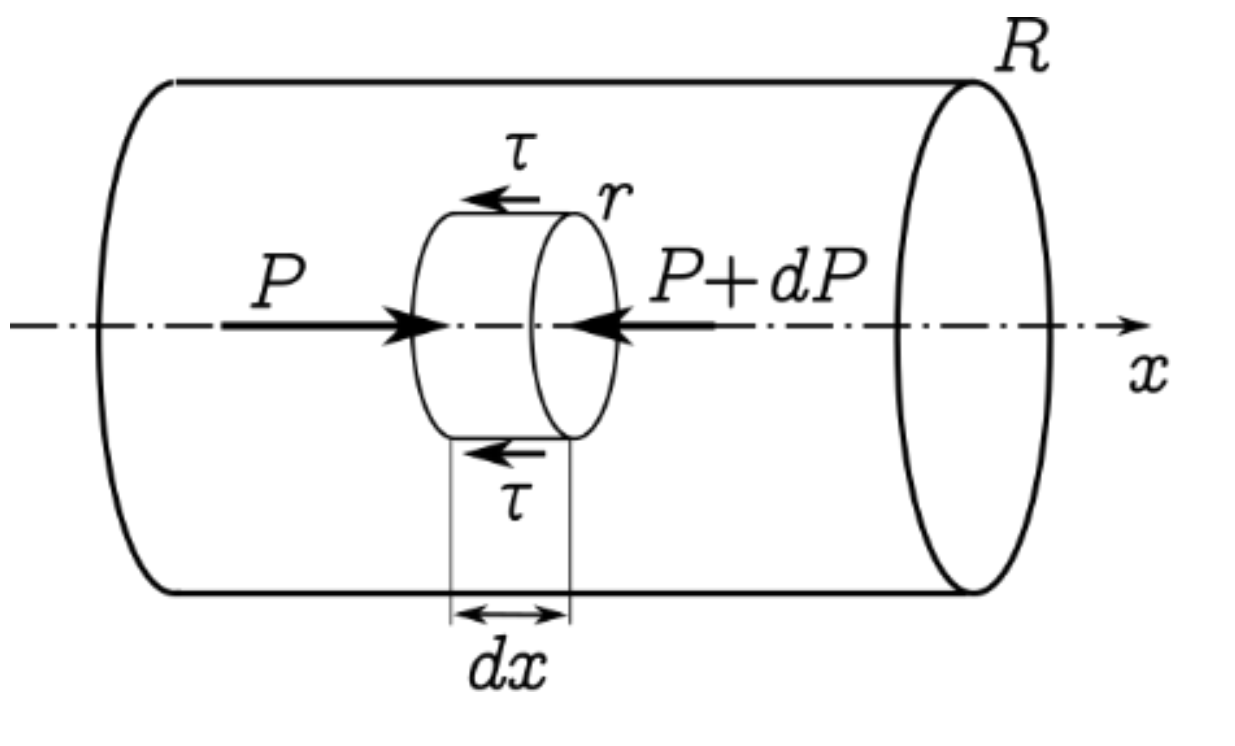
\includegraphics[scale=0.5]{Puaseil.png}
        \caption{
        Рис. 1. К выводу формулы Пуазейля
        }
 \end{figure}
Выделим соосный трубе цилиндр некоторого радиуса $r$ и длины $dx$ (см.
Рис. 1). Поскольку при стационарном течении жидкость течёт без ускорения,
сумма всех сил, действующих на жидкость в цилиндре, должна быть равна
нулю. На жидкость внутри цилиндра действует направленная вдоль оси трубы
сила
\begin{equation*}
	F_{1x} = -\pi r^2dP,
\end{equation*}
где $dP = P(x + dx) - P(x) < 0$ - разность давлений в сечениях на торцах
выделенного участка. На боковые поверхности цилиндра действует касательная сила вязкого трения
\begin{equation*}
	F_{2x} = -\tau 2\pi rdx,
\end{equation*}
где согласно закону Ньютона касательное напряжение равно
\begin{equation*}
	\tau = -\eta \frac{du}{dr}.
\end{equation*}
Из условия баланса сил $F_{1x} + F_{2x} = $ находим
\begin{equation*}
	\frac{dP}{dx} = -\eta \frac{2du}{rdr}
\end{equation*}
В установившемся течении правая часть полученного выражения является
функцией только радиуса $r$. В левой части находится градиент давления,
который не зависит от $r$ вовсе, и, следовательно, обе части уравнения являются константами. Тогда, проводя интегрирование, приходим к следующему. Во-первых, давление в трубе является линейно убывающей функцией координаты
\begin{equation*}
	P(x) = P_0 - \frac{\Delta P}{l}x,
\end{equation*}
где $\Delta P$ — перепад давления на участке длиной $l$, $P_0$ — давление в начале
участка (в точке $x = 0$). Во-вторых, профиль скорости является параболической функцией с максимумом на оси трубы
\begin{equation*}
	u(r) = u_{max} - \frac{\Delta P}{4l}r^2.
\end{equation*}
В рассматриваемой задаче стенки неподвижны, поэтому имеем
\begin{equation*}
	\left. u(r) \right|_{r = R} = 0,
\end{equation*}
\begin{equation*}
	u_{max} = \frac{\Delta P}{4l}R^2.
\end{equation*}
\begin{equation*}
	u(r) = \frac{\Delta P}{4l}(R^2 - r^2)
\end{equation*}
интегрируя $u(r)$по сечению трубы, получим объёмный расход жидкости в зависимости от перепада давления на концах:
\begin{equation*}
	Q = \int_{0}^{R} u(r) \cdot 2\pi r\, dr = \frac{\pi R^4 \Delta P}{8\eta l}.
	\eqno(1)
\end{equation*}
Это соотношение называют формулой Пуазейля. Заметим, что средняя скорость потока при пуазейлевском течении, как видно из (1), оказывается
вдвое меньше максимальной:
\begin{equation*}
	\bar{u} \equiv \frac{Q}{\pi R^2} = \frac{u_{max}}{2}.
\end{equation*}
\subsection{Вязкость газов}
Рассмотрим механизм возникновения вязкости в газах.
Молекулы газа участвуют как в направленном движении со средней скоростью потока $u$, так и в хаотическом тепловом движении, характеризующимся
средней тепловой скоростью $\bar{v} = \sqrt{\frac{8k_{\text{Б}}T}{\pi m}}$ (здесь $m$ — масса молекулы). Молекулы могут свободно перемещаться между слоями и обмениваться друг с другом импульсами при столкновениях. Если в двух соседних слоях потоковыескорости различны, то такой обмен импульсом и приводит к эффективному возникновению силы трения между слоями. Исходя из приведенных соображений можно получить следующую
оценку для коэффициента вязкости идеального газа:
\begin{equation*}
	\eta \sim \frac{1}{3}\rho \bar{v} \lambda,
	\eqno(2)
\end{equation*}
где $\lambda$ — длина свободного пробега молекул газа относительно столкновений
друг с другом. Как известно из молекулярно-кинетической теории, длина пробега определяется эффективным («газокинетическим») диаметром молекул $d$
как $\lambda \sim 1/(n\pi d^2)$, где $n$ — объёмная концентрация газа. Видно, что $\lambda$ обратно пропорциональна плотности газа, поэтому, как следует из (2), вязкость газа не
зависит от его плотности и определяется только температурой $T$. Данный
вывод может показаться парадоксальным, поскольку в более плотном газе
большее число молекул должно участвовать в передаче импульса между слоями, однако это компенсируется тем, что этот импульс передается на меньшее
расстояние.

\subsection{Оценка турбулентного течения}
В качестве примера воспользуемся аналогией с молекулярно-кинетической теорией и рассмотрим следующую упрощенную модель турбулентного
течения. Примем, что флуктуации скорости в развитом турбулентном течении
по порядку величины совпадают со средней скоростью потока $u \sim \bar{u}$. При
этом элементы жидкости практически равномерно перемешиваются по сечению трубы, так что в качестве «длины пробега» жидкой частицы можно взять поперечный размер системы $R$. Тогда по аналогии с формулой (2) определим «турбулентную вязкость» как
\begin{equation*}
	\eta_{\text{турб}} \sim \rho \bar{u} R.
	\eqno(3)
\end{equation*}
Далее по аналогии с выводом формулы Пуазейля запишем баланс сил в потоке, откуда получим оценку для средней скорости течения:
\begin{equation*}
	\eta_{\text{турб}}\frac{\bar{u}}{R} \cdot 2\pi rl \sim \pi R^2 \Delta P,
\end{equation*}
\begin{equation*}
	\bar{u} \sim \frac{R^2 \Delta P}{\eta_{\text{турб}} l}.
\end{equation*}
Подставляя сюда (3), находим скорость $\bar{u} \sim \sqrt{\frac{R \Delta P}{\rho l}}$
и, как следствие, расход:
\begin{equation*}
	Q = \pi R^2 \bar{u} \sim R^{5/2}\sqrt{\frac{\Delta P}{\rho l}}.
	\eqno(4)
\end{equation*}
Заметим, что эта теоретическая модель довольно груба и никак не учитывает сложную структуру турбулентного течения (например, не учитывается зависимость скорости потока $u$ от расстояния $r$ до оси трубы). 


\section{Экспериментальная установка}
Схема экспериментальной установки изображена на Рис. 2. Поток воздуха
под давлением, немного превышающим атмосферное, поступает через газовый счётчик в тонкие металлические трубки. Воздух нагнетается компрессором, интенсивность его подачи регулируется краном К. Трубки снабжены
съёмными заглушками на концах и рядом миллиметровых отверстий, к которым можно подключать микроманометр. В рабочем состоянии открыта заглушка на одной (рабочей) трубке, микроманометр подключён к двум её выводам, а все остальные отверстия плотно закрыты пробками.
Перед входом в газовый счётчик установлен водяной U-образный манометр. Он служит для измерения давления газа на входе, а также предохраняет
счётчик от выхода из строя. При превышении максимального избыточного
давления на входе счётчика ($\sim$ 30 см вод. ст.) вода выплёскивается из трубки
в защитный баллон Б, создавая шум и привлекая к себе внимание экспериментатора.
\begin{figure}[h!]
        \centering
        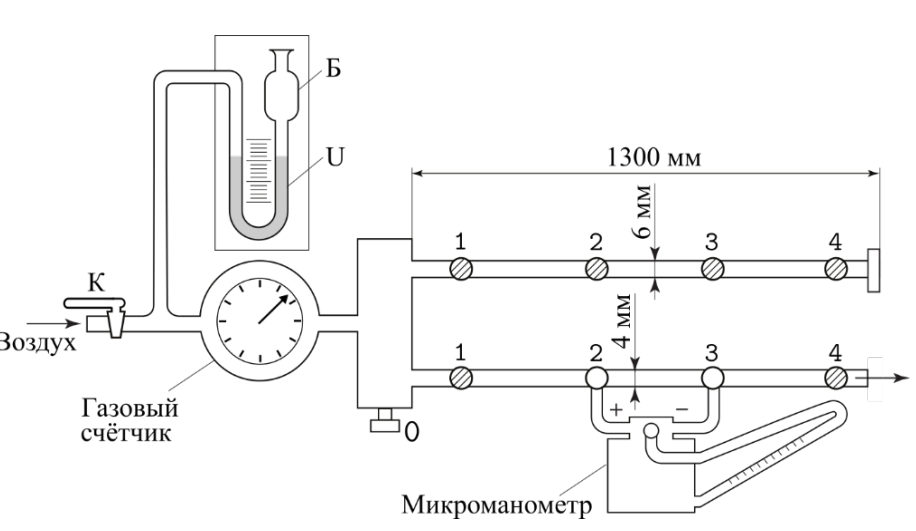
\includegraphics[scale=0.5]{Ustanovka.png}
        \caption{
        Рис. 2. Экспериментальная установка
        }
 \end{figure} 

\section{Приборы и данные}
\begin{itemize}
    \item Счетчик газовый барабанный модель ВИКС-1, погрешность измерения 1\%
    \item Термогигрометр с функцией отображения давления testo 622, погрешность измерения давления 3 гПа, температуры - 0,4 $^\circ C$, влажности - 2\% в диапазоне от 0 до 90 \%
    \item Микроманометр ММН-2400(5)-1б0, погрешность при различных K: 6 Па ($K = 0,2$), 9 Па ($K = 0,3$), 12 Па ($K = 0,4$), 18 Па ($K = 0,6$).
\end{itemize}

\section{Выполнение}
\begin{enumerate}

\item Начальные показания 
\begin{equation*}
	t_\text{н} = 27,7 ^\circ C,
\end{equation*}
\begin{equation*}
	P_\text{н} = 996,9 \text{ гПа},
\end{equation*}
\begin{equation*}
	\varphi_\text{н} = 23,3 \%.
\end{equation*}
Показания в конце эксперимента
\begin{equation*}
	t_\text{к} = 27,3 ^\circ C,
\end{equation*}
\begin{equation*}
	P_\text{к} = 996,3 \text{ гПа},
\end{equation*}
\begin{equation*}
	\varphi_\text{к} = 21,2 \%.
\end{equation*}
где $t$ - температруа в комнате, $P$ - давление, $\varphi$ - относительная влажность.\\
С учетом этих данных плотность спирта (концентрация 96\%) бралась средняя между $\rho_{27} = 0,80123 \frac{\text{г}}{\text{см}^3}$ и $\rho_{28} = 0,80043 \frac{\text{г}}{\text{см}^3}$ ($\rho_{\text{сп.залит.}} = 0,80083 \frac{\text{г}}{\text{см}^3}$).

\item Предварительные оценки\\
Оценим критический расход и перепад давлений для каждой трубки. Для этого примем вязкость воздуха $\eta = 2 \cdot 10^{-5} \text{Па}\cdot \text{с}$, число Рейнольдса $Re_\text{кр} \approx 10^3$. Первая трубка диаметром $3,90 \pm 0,05$ мм:\\
\begin{equation*}
    Q_\text{кр}^1 = \frac{\pi Re_\text{кр} R_{\text{газ}} T \eta R}{P \mu_{\text{воз}}} = \frac{3,1415 \cdot 10^3 \cdot8,31 \cdot 300,7 \cdot 2 \cdot10^{-5}\cdot \frac{3,9}{2} \cdot 10^{-3}}{99690 \cdot29 \cdot 10^{-3}} \approx 1,06 \cdot 10^{-4} \frac{\text{ м}^3}{c} = 6,35 \frac{\text{л}}{\text{мин}},
\end{equation*}
1. $l = 0,5 \text{ м}$

\begin{equation*}
    \Delta P_\text{кр}^1 = \frac{8 Q_\text{кр}^1 \eta l}{\pi R^4} = \frac{8 \cdot 1,06 \cdot 10^{-4}\cdot 2 \cdot10^{-5} \cdot 0,5}{3,1415 \cdot (\frac{3,9}{2}\cdot 10^{-3})^4} \approx 187 \text{ Па}.
\end{equation*}

2. $l = 0,9 \text{ м}$: $\Delta P_\text{кр}^2 \approx 337 \text{ Па}. $

3. $l = 1,2 \text{ м}$: $\Delta P_\text{кр}^3 \approx 449 \text{ Па}. $

Вторая трубка диаметром $5,25 \pm 0,05$ мм: $Q_\text{кр}^2 \approx 8,55  \frac{\text{л}}{\text{мин}}$.\\
1. $l = 0,5 \text{ м}$: $ \Delta P_\text{кр}^4 =  \approx 77 \text{ Па}.$

2. $l = 0,4 \text{ м}$: $\Delta P_\text{кр}^5 \approx 62 \text{ Па}. $

3. $l = 0,3 \text{ м}$: $\Delta P_\text{кр}^6 \approx 46 \text{ Па}. $

Третья трубка диаметром $3,0 \pm 0,1$ мм: $Q_\text{кр}^3 \approx 4,89  \frac{\text{л}}{\text{мин}}$.\\
1. $l = 0,2 \text{ м}$: $\Delta P_\text{кр}^7 =  \approx 164 \text{ Па}.$

2. $l = 0,4 \text{ м}$: $\Delta P_\text{кр}^8 \approx 329 \text{ Па}. $

Оценим длину установления давления в трубках.
Первая трубка диаметром $3,90 \pm 0,05$ мм:\\
\begin{equation*}
    \l_{\text{уст}}^1 \approx 0,2 Re_\text{кр} R \approx 0,39 \text{ м}
\end{equation*}
Вторая трубка диаметром $5,25 \pm 0,05$ мм:\\
\begin{equation*}
    \l_{\text{уст}}^2 \approx 0,53 \text{ м}
\end{equation*}
Третья трубка диаметром $3,0 \pm 0,1$ мм:\\
\begin{equation*}
    \l_{\text{уст}}^3 \approx 0,30 \text{ м}
\end{equation*}

\item Для трех трубок разных диаметров, меняя расположение микроманометра по длине трубки, будем менять расход сначала в пределах, когда течение еще ламинарное, а затем для турбулентного. Для каждого расхода будем фиксировать перепад давления. 
Данные для ламинарных течений в левой колонке, для турбулентных течений - в правой.
\clearpage
\begin{multicols}{2}
%\scriptsize
\begin{center}
    \begin{tabular}{|c|c|c|c|}
        \hline
        $Q, \frac{\text{л}}{\text{мин}} $& $\sigma_Q, \frac{\text{л}}{\text{мин}} $& $\Delta P \pm \sigma_{\Delta P}$, Па & $\varepsilon_{\Delta P}$, \% \\
        \hline
        1.352 & 0.014 & $37 \pm 6$ & 16.2 \\ \hline
        2.363 & 0.024 & $64 \pm 6$ & 9.3 \\ \hline
        2.894 & 0.029 & $78 \pm 6$ & 7.7 \\ \hline
        3.897 & 0.039 & $107 \pm 6$ & 5.6 \\ \hline
        4.468 & 0.045 & $134 \pm 6$ & 4.5 \\ \hline
        4.945 & 0.049 & $140 \pm 6$ & 4.3 \\ \hline
        5.483 & 0.055 & $162 \pm 6$ & 3.7 \\ \hline
    \end{tabular}
    \captionof{table}{Таблица 1. $d = 3,90 \pm 0,05$ мм; $l = 0,5$ м; $K = 0,2$}
\end{center}
\vspace{1em}
\begin{center}
    \begin{tabular}{|c|c|c|c|}
        \hline
         $Q, \frac{\text{л}}{\text{мин}} $& $\sigma_Q, \frac{\text{л}}{\text{мин}} $& $\Delta P \pm \sigma_{\Delta P}$, Па & $\varepsilon_{\Delta P}$, \% \\
        \hline
        1.28 & 0.013 & $58 \pm 9$ & 15.4 \\ \hline
        2.788 & 0.028 & $120 \pm 9$ & 7.5 \\ \hline
        3.226 & 0.032 & $158 \pm 9$ & 5.7 \\ \hline
        3.581 & 0.036 & $175 \pm 9$ & 5.1 \\ \hline
        4.138 & 0.041 & $201 \pm 9$ & 4.5 \\ \hline
        4.58 & 0.046 & $210 \pm 9$ & 4.3 \\ \hline
        5.04 & 0.050 & $257 \pm 9$ & 3.5 \\ \hline
        5.452 & 0.055 & $292 \pm 9$ & 3.1 \\ \hline
    \end{tabular}
    \captionof{table}{Таблица 2. $d = 3,90 \pm 0,05$ мм; $l = 0,9$ м; $K = 0,3$}
\end{center}
\vspace{1em}
\begin{center}
    \begin{tabular}{|c|c|c|c|}
        \hline
         $Q, \frac{\text{л}}{\text{мин}} $& $\sigma_Q, \frac{\text{л}}{\text{мин}} $& $\Delta P \pm \sigma_{\Delta P}$, Па & $\varepsilon_{\Delta P}$, \% \\
        \hline
        1.024 & 0.010 & $62 \pm 12$ & 19.2 \\ \hline
        2.236 & 0.022 & $140 \pm 12$ & 8.6 \\ \hline
        2.584 & 0.026 & $168 \pm 12$ & 7.2 \\ \hline
        3.212 & 0.032 & $206 \pm 12$ & 5.8 \\ \hline
        3.621 & 0.036 & $234 \pm 12$ & 5.1 \\ \hline
        4.404 & 0.044 & $292 \pm 12$ & 4.1 \\ \hline
        5.166 & 0.052 & $355 \pm 12$ & 3.4 \\ \hline
    \end{tabular}
    \captionof{table}{Таблица 3. $d = 3,90 \pm 0,05$ мм; $l = 1,2$ м; $K = 0,4$}
\end{center}
\vspace{1em}
\begin{center}
    \begin{tabular}{|c|c|c|c|}
        \hline
         $Q, \frac{\text{л}}{\text{мин}} $& $\sigma_Q, \frac{\text{л}}{\text{мин}} $& $\Delta P \pm \sigma_{\Delta P}$, Па & $\varepsilon_{\Delta P}$, \% \\
        \hline
        2.58 & 0.026 & $19 \pm 6$ & 30.8 \\ \hline
        3.31 & 0.033 & $27 \pm 6$ & 22.0 \\ \hline
        5.399 & 0.054 & $45 \pm 6$ & 13.4 \\ \hline
        6.638 & 0.066 & $55 \pm 6$ & 11.0 \\ \hline
        4.485 & 0.045 & $37 \pm 6$ & 16.2 \\ \hline
        6.91 & 0.069 & $58 \pm 6$ & 10.3 \\ \hline
        5.116 & 0.051 & $43 \pm 6$ & 14.0 \\ \hline
    \end{tabular}
    \captionof{table}{Таблица 4. $d = 5,25 \pm 0,05$ мм; $l = 0,5$ м; $K = 0,2$}
\end{center}
\vspace{1em}
\begin{center}
    \begin{tabular}{|c|c|c|c|}
        \hline
         $Q, \frac{\text{л}}{\text{мин}} $& $\sigma_Q, \frac{\text{л}}{\text{мин}} $& $\Delta P \pm \sigma_{\Delta P}$, Па & $\varepsilon_{\Delta P}$, \% \\
        \hline
        2.478 & 0.025 & $16 \pm 6$ & 38.5 \\ \hline
        3.383 & 0.034 & $23 \pm 6$ & 25.7 \\ \hline
        5.441 & 0.054 & $39 \pm 6$ & 15.4 \\ \hline
        4.226 & 0.042 & $29 \pm 6$ & 20.5 \\ \hline
        6.386 & 0.064 & $47 \pm 6$ & 12.8 \\ \hline
        6.964 & 0.070 & $51 \pm 6$ & 11.8 \\ \hline
        7.815 & 0.078 & $58 \pm 6$ & 10.3 \\ \hline
    \end{tabular}
    \captionof{table}{Таблица 5. $d = 5,25 \pm 0,05$ мм; $l = 0,4$ м; $K = 0,2$}
\end{center}
\vspace{1em}
\begin{center}
    \begin{tabular}{|c|c|c|c|}
        \hline
        $Q, \frac{\text{л}}{\text{мин}}$ & $\sigma_Q, \frac{\text{л}}{\text{мин}}$ & $\Delta P \pm \sigma_{\Delta P}$, Па & $\varepsilon_{\Delta P}$, \% \\
        \hline
	   7,083 & 0,071 & 308\footnotemark[1] $\pm 6$ & 1,9 \\ \hline
        7.943 & 0.079 & $385 \pm 9$ & 2.3 \\ \hline
        8.533 & 0.085 & $447 \pm 9$ & 2.0 \\ \hline
        9.395 & 0.094 & $540 \pm 9$ & 1.7 \\ \hline
        9.814 & 0.098 & $587 \pm 9$ & 1.5 \\ \hline
        10.052 & 0.101 & $610 \pm 9$ & 1.5 \\ \hline
        10.755 & 0.108 & $701 \pm 9$ & 1.3 \\ \hline
    \end{tabular}
    \captionof{table}{Таблица 9. $d = 3,90 \pm 0,05$ мм; $l = 0,5$ м; $K = 0,3$}
\end{center}
\vspace{1em}
\footnotetext[1]{Это давление рассчитывалось с $K = 0.2$, остальные с 0.3}
\begin{center}
    \begin{tabular}{|c|c|c|c|}
        \hline
        $Q, \frac{\text{л}}{\text{мин}}$ & $\sigma_Q, \frac{\text{л}}{\text{мин}}$ & $\Delta P \pm \sigma_{\Delta P}$, Па & $\varepsilon_{\Delta P}$, \% \\
        \hline
        7.058 & 0.071 & $510 \pm 12$ & 2.4 \\ \hline
        7.799 & 0.078 & $686 \pm 12$ & 1.7 \\ \hline
        8.452 & 0.085 & $791 \pm 12$ & 1.5 \\ \hline
        8.793 & 0.088 & $857 \pm 12$ & 1.4 \\ \hline
        9.087 & 0.091 & $927 \pm 12$ & 1.3 \\ \hline
        9.319 & 0.093 & $978 \pm 12$ & 1.2 \\ \hline
        9.814 & 0.098 & $1064 \pm 12$ & 1.1 \\ \hline
    \end{tabular}
    \captionof{table}{\\Таблица 10. $d = 3,90 \pm 0,05$ мм; $l = 0,9$ м; $K = 0,4$}
\end{center}


\vspace{1em}
\begin{center}
    \begin{tabular}{|c|c|c|c|}
        \hline
        $Q, \frac{\text{л}}{\text{мин}}$ & $\sigma_Q, \frac{\text{л}}{\text{мин}}$ & $\Delta P \pm \sigma_{\Delta P}$, Па & $\varepsilon_{\Delta P}$, \% \\
        \hline
        7.632 & 0.076 & $839 \pm 18$ & 2.1 \\ \hline
        8.113 & 0.081 & $950 \pm 18$ & 1.9 \\ \hline
        8.441 & 0.084 & $1020 \pm 18$ & 1.8 \\ \hline
        8.895 & 0.089 & $1125 \pm 18$ & 1.6 \\ \hline
        9.575 & 0.096 & $1288 \pm 18$ & 1.4 \\ \hline
        9.313 & 0.093 & $1235 \pm 18$ & 1.5 \\ \hline
        9.868 & 0.099 & $1398 \pm 18$ & 1.3 \\ \hline
    \end{tabular}
    \captionof{table}{Таблица 11. $d = 3,90 \pm 0,05$ мм; $l = 1,2$ м; $K = 0,6$}
\end{center}
\vspace{1em}
\begin{center}
    \begin{tabular}{|c|c|c|c|}
        \hline
        $Q, \frac{\text{л}}{\text{мин}}$ & $\sigma_Q, \frac{\text{л}}{\text{мин}}$ & $\Delta P \pm \sigma_{\Delta P}$, Па & $\varepsilon_{\Delta P}$, \% \\
        \hline
        9.067 & 0.091 & $109 \pm 6$ & 5.5 \\ \hline
        9.735 & 0.097 & $134 \pm 6$ & 4.5 \\ \hline
        10.334 & 0.103 & $156 \pm 6$ & 3.8 \\ \hline
        11.379 & 0.114 & $185 \pm 6$ & 3.2 \\ \hline
        12.416 & 0.124 & $218 \pm 6$ & 2.7 \\ \hline
        13.158 & 0.132 & $249 \pm 6$ & 2.4 \\ \hline
        13.935 & 0.139 & $267 \pm 6$ & 2.2 \\ \hline
    \end{tabular}
    \captionof{table}{Таблица 12. $d = 5,25 \pm 0,05$ мм; $l = 0,5$ м; $K = 0,2$}
\end{center}
\vspace{1em}
\begin{center}
    \begin{tabular}{|c|c|c|c|}
        \hline
        $Q, \frac{\text{л}}{\text{мин}}$ & $\sigma_Q, \frac{\text{л}}{\text{мин}}$ & $\Delta P \pm \sigma_{\Delta P}$, Па & $\varepsilon_{\Delta P}$, \% \\
        \hline
        9.305 & 0.093 & $103 \pm 6$ & 5.8 \\ \hline
        10.103 & 0.101 & $127 \pm 6$ & 4.7 \\ \hline
        11.228 & 0.112 & $154 \pm 6$ & 3.9 \\ \hline
        11.921 & 0.119 & $173 \pm 6$ & 3.5 \\ \hline
        12.679 & 0.127 & $193 \pm 6$ & 3.1 \\ \hline
        13.052 & 0.131 & $205 \pm 6$ & 2.9 \\ \hline
        13.583 & 0.136 & $222 \pm 6$ & 2.7 \\ \hline
    \end{tabular}
    \captionof{table}{Таблица 13. $d = 5,25 \pm 0,05$ мм; $l = 0,4$ м; $K = 0,2$}
\end{center}
\vspace{1em}
\end{multicols}
\begin{multicols}{2}
\begin{center}
    \begin{tabular}{|c|c|c|c|}
        \hline
         $Q, \frac{\text{л}}{\text{мин}} $& $\sigma_Q, \frac{\text{л}}{\text{мин}} $& $\Delta P \pm \sigma_{\Delta P}$, Па & $\varepsilon_{\Delta P}$, \% \\
        \hline
        1.535 & 0.015 & $8 \pm 6$ & 77.0 \\ \hline
        2.738 & 0.027 & $14 \pm 6$ & 44.0 \\ \hline
        3.759 & 0.038 & $19 \pm 6$ & 30.8 \\ \hline
        4.331 & 0.043 & $23 \pm 6$ & 25.7 \\ \hline
        4.922 & 0.049 & $27 \pm 6$ & 22.0 \\ \hline
        6.245 & 0.062 & $35 \pm 6$ & 17.1 \\ \hline
        6.811 & 0.068 & $39 \pm 6$ & 15.4 \\ \hline
    \end{tabular}
    \captionof{table}{Таблица 6. $d = 5,25 \pm 0,05$ мм; $l = 0,3$ м; $K = 0,2$}
\end{center}
\vspace{1em}
\begin{center}
    \begin{tabular}{|c|c|c|c|}
        \hline
         $Q, \frac{\text{л}}{\text{мин}} $& $\sigma_Q, \frac{\text{л}}{\text{мин}} $& $\Delta P \pm \sigma_{\Delta P}$, Па & $\varepsilon_{\Delta P}$, \% \\
        \hline
        1.118 & 0.011 & $10 \pm 6$ & 61.6 \\ \hline
        1.901 & 0.019 & $19 \pm 6$ & 30.8 \\ \hline
        1.26 & 0.013 & $12 \pm 6$ & 51.3 \\ \hline
        1.54 & 0.015 & $14 \pm 6$ & 44.0 \\ \hline
        2.347 & 0.023 & $23 \pm 6$ & 25.7 \\ \hline
        2.733 & 0.027 & $29 \pm 6$ & 20.5 \\ \hline
        3.197 & 0.032 & $37 \pm 6$ & 16.2 \\ \hline
    \end{tabular}
    \captionof{table}{Таблица 7. $d = 3,0 \pm 0,1$ мм; $l = 0,2$ м; $K = 0,2$}
\end{center}
\vspace{1em}
\begin{center}
    \begin{tabular}{|c|c|c|c|}
        \hline
        $Q, \frac{\text{л}}{\text{мин}} $& $\sigma_Q, \frac{\text{л}}{\text{мин}} $& $\Delta P \pm \sigma_{\Delta P}$, Па & $\varepsilon_{\Delta P}$, \% \\
        \hline
        0.561 & 0.006 & $12 \pm 6$ & 51.3 \\ \hline
        1.107 & 0.011 & $25 \pm 6$ & 23.7 \\ \hline
        1.574 & 0.016 & $39 \pm 6$ & 15.4 \\ \hline
        1.86 & 0.019 & $47 \pm 6$ & 12.8 \\ \hline
        2.135 & 0.021 & $51 \pm 6$ & 11.8 \\ \hline
    \end{tabular}
    \captionof{table}{Таблица 8. $d = 3,0 \pm 0,1$ мм; $l = 0,4$ м; $K = 0,2$}
\end{center}
\vspace{1em}
\begin{center}
    \begin{tabular}{|c|c|c|c|}
        \hline
        $Q, \frac{\text{л}}{\text{мин}}$ & $\sigma_Q, \frac{\text{л}}{\text{мин}}$ & $\Delta P \pm \sigma_{\Delta P}$, Па & $\varepsilon_{\Delta P}$, \% \\
        \hline
        10.947 & 0.109 & $92 \pm 6$ & 6.6 \\ \hline
        11.684 & 0.117 & $103 \pm 6$ & 5.8 \\ \hline
        12.177 & 0.122 & $113 \pm 6$ & 5.3 \\ \hline
        12.662 & 0.127 & $119 \pm 6$ & 5.0 \\ \hline
        13.137 & 0.131 & $129 \pm 6$ & 4.7 \\ \hline
        13.591 & 0.136 & $136 \pm 6$ & 4.4 \\ \hline
        14.102 & 0.141 & $144 \pm 6$ & 4.2 \\ \hline
    \end{tabular}
    \captionof{table}{Таблица 14. $d = 5,25 \pm 0,05$ мм; $l = 0,3$ м; $K = 0,2$}
\end{center}
\vspace{1em}
\begin{center}
    \begin{tabular}{|c|c|c|c|}
        \hline
        $Q, \frac{\text{л}}{\text{мин}}$ & $\sigma_Q, \frac{\text{л}}{\text{мин}}$ & $\Delta P \pm \sigma_{\Delta P}$, Па & $\varepsilon_{\Delta P}$, \% \\
        \hline
        6.038 & 0.060 & $97 \pm 6$ & 6.2 \\ \hline
        6.803 & 0.068 & $113 \pm 6$ & 5.3 \\ \hline
        7.139 & 0.071 & $125 \pm 6$ & 4.8 \\ \hline
        8.375 & 0.084 & $156 \pm 6$ & 3.8 \\ \hline
        8.966 & 0.090 & $175 \pm 6$ & 3.4 \\ \hline
        9.56 & 0.096 & $203 \pm 6$ & 3.0 \\ \hline
        10.179 & 0.102 & $222 \pm 6$ & 2.7 \\ \hline
    \end{tabular}
    \captionof{table}{Таблица 15. $d = 3,0 \pm 0,1$ мм; $l = 0,2$ м; $K = 0,2$}
\end{center}
\vspace{1em}
\begin{center}
    \begin{tabular}{|c|c|c|c|}
        \hline
        $Q, \frac{\text{л}}{\text{мин}}$ & $\sigma_Q, \frac{\text{л}}{\text{мин}}$ & $\Delta P \pm \sigma_{\Delta P}$, Па & $\varepsilon_{\Delta P}$, \% \\
        \hline
        5.202 & 0.052 & $187 \pm 6$ & 3.2 \\ \hline
        5.836 & 0.058 & $228 \pm 6$ & 2.6 \\ \hline
        6.194 & 0.062 & $245 \pm 6$ & 2.4 \\ \hline
        6.951 & 0.070 & $310 \pm 6$ & 1.9 \\ \hline
        7.662 & 0.077 & $364 \pm 6$ & 1.6 \\ \hline
    \end{tabular}
    \captionof{table}{Таблица 16. $d = 3,0 \pm 0,1$ мм; $l = 0,4$ м; $K = 0,2$}
\end{center}
\end{multicols}
\item Для каждой серии построим график зависимости $Q(\Delta P)$ по методу $\chi^2$.
Введем обозначения\\
$w_i = \frac{1}{\sigma_i^2}\text{ - веса}$, $S = \displaystyle \sum_{i=1}^{n} w_i$, $S_x = \displaystyle \sum_{i=1}^{n} w_ix_i$, $S_y = \displaystyle \sum_{i=1}^{n} w_iy_i$, $S_{x^2} = \displaystyle \sum_{i=1}^{n} w_ix_i^2$, $S_{xy} = \displaystyle \sum_{i=1}^{n} w_ix_iy_i$.

Тогда параметры $a$ и $b$ прямой $y = ax + b$ находятся как:
\begin{equation*}
	a = \frac{S \cdot S_{xy} - S_x \cdot S_y}{S \cdot S_{x^2} - S_x^2},
\end{equation*}
\begin{equation*}
	b = \frac{S_{x^2} \cdot S_{y} - S_x \cdot S_{xy}}{S \cdot S_{x^2} - S_x^2}.
\end{equation*}
Погрешности коэффициентов выражаются так:
\begin{equation*}
	\sigma_a^2 = \frac{S}{S \cdot S_{x^2} - S_x^2},
\end{equation*}
\begin{equation*}
	\sigma_b^2 = \frac{S_{x^2}}{S \cdot S_{x^2} - S_x^2}.
\end{equation*}
\begin{equation*}
	\chi^2 = \sum_{i=1}^{n} \left(\frac{y_i - ax_i-b}{\sigma_i}\right)^2
\end{equation*}
Величина $\frac{\chi^2}{dof}$, где $dof$ (degrees of freedom) равно к $n-2$ (количество точек минус количество параметров) характеризует степень согласия модели с данными. Если $\frac{\chi^2}{dof} \approx 1$, это означает хорошее согласие.\\
$p$-value - это уровень значимости, статистический показатель. Это вероятность того, что нормально распределённая случайная величина примет значение больше по модулю, чем наблюдаемое. Если $p-value < 0.05$, это значит что данная модель плохо подходит для описания данных.\\
Теперь перейдем к графикам
\clearpage
\begin{figure}[h!]
\centering{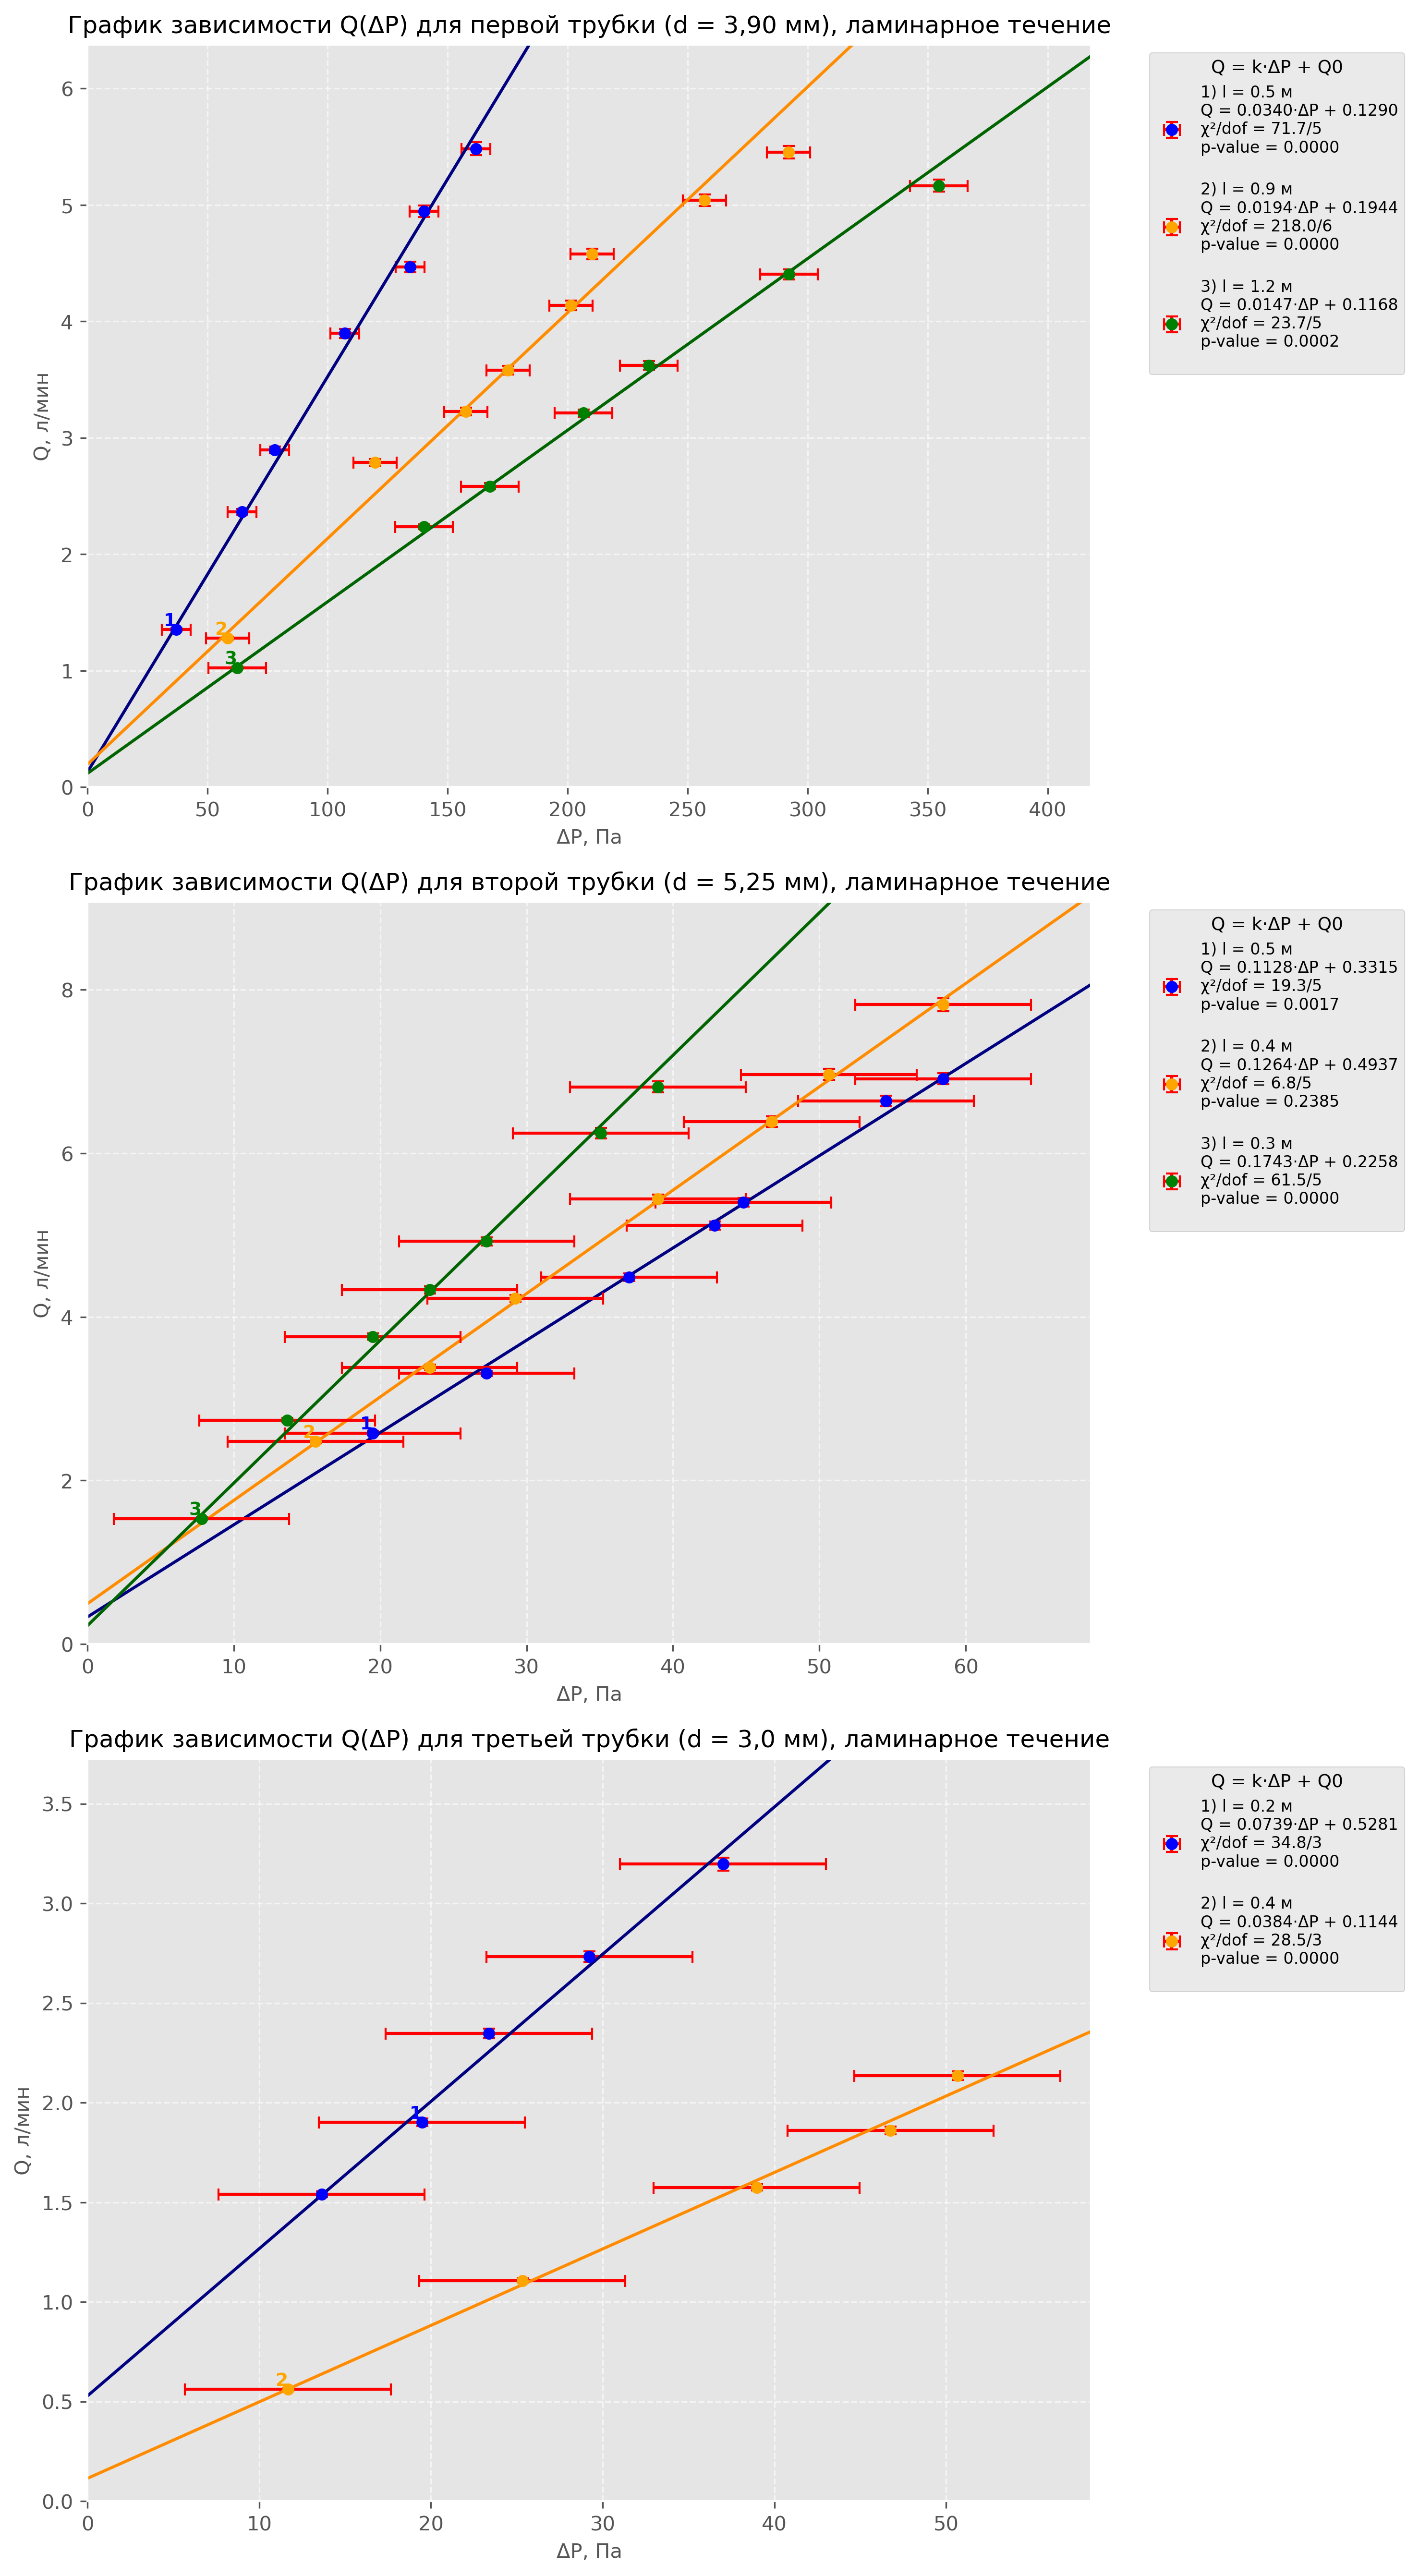
\includegraphics[width=0.75\textwidth]{Graph_1-3_lam.png}}
\caption[]{\label{} Графики №1-3 Линейная зависимость $Q(\Delta P)$ при ламинарном течении}
\end{figure}
\clearpage
\begin{figure}[h!]
\centering{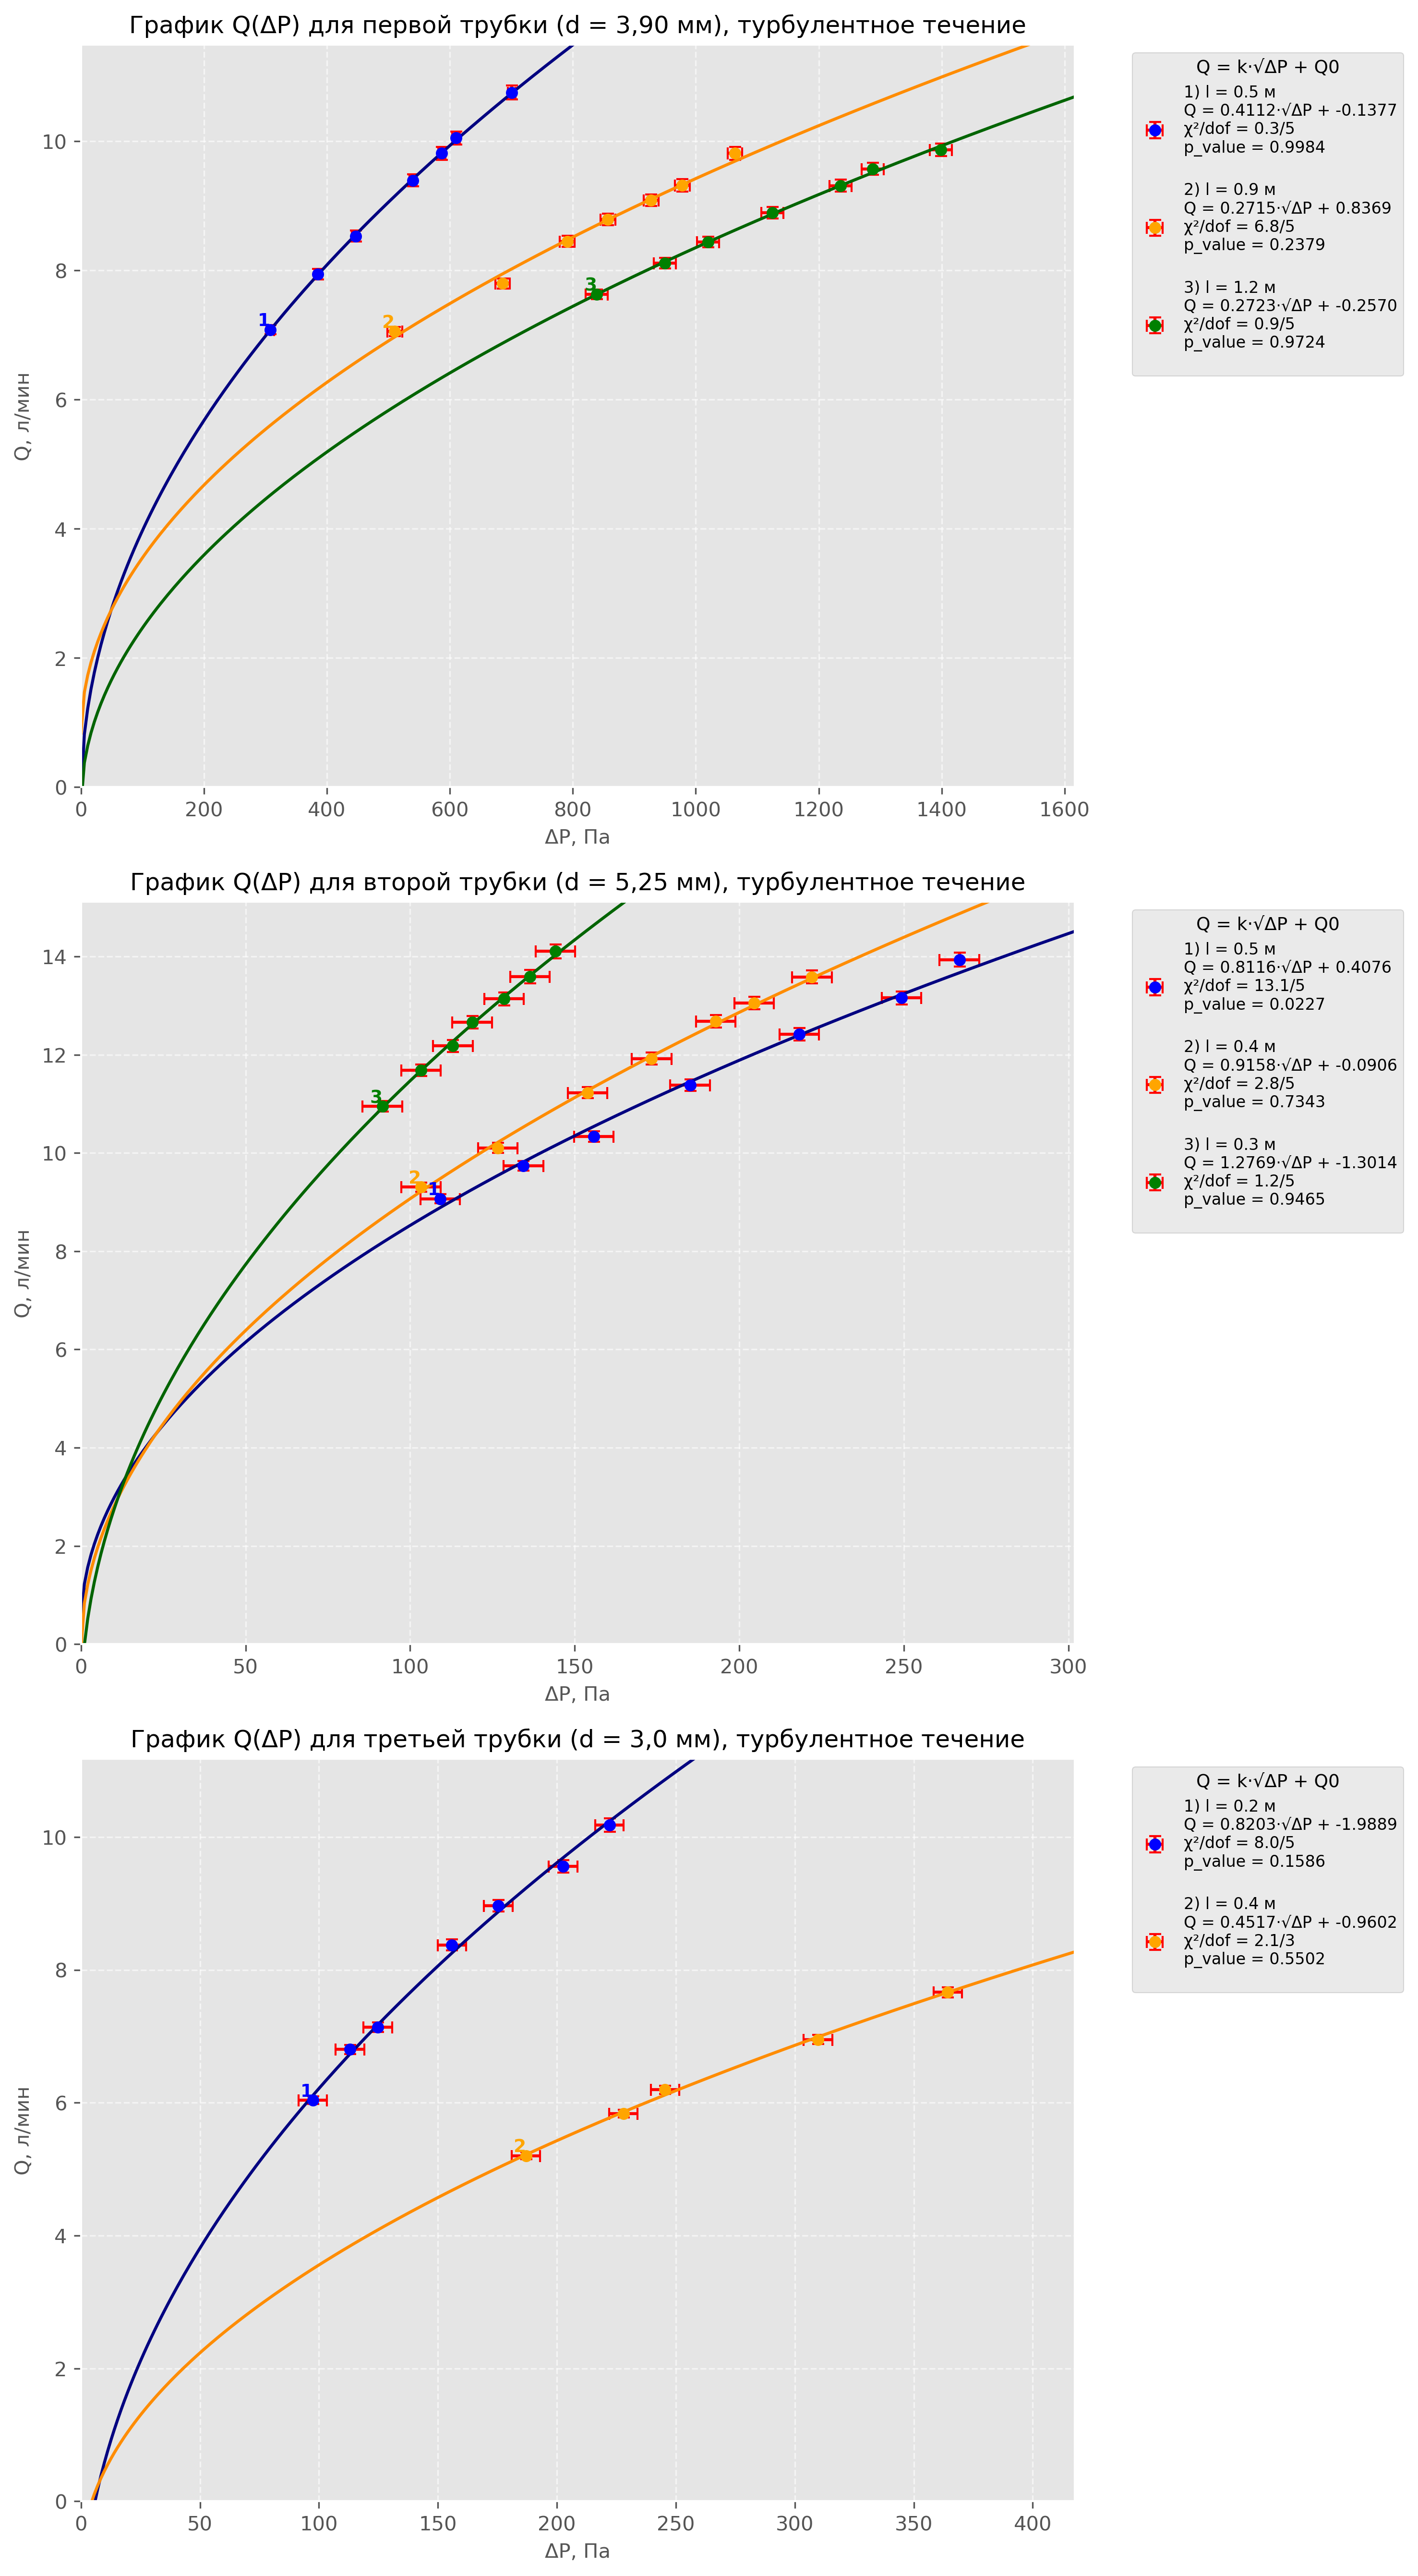
\includegraphics[width=0.75\textwidth]{Graph_4-6_tur.png}}
\caption[]{\label{} Графики №4-6 Коренная зависимость $Q(\Delta P)$ при турбулентном течении}
\end{figure}
\clearpage
\begin{figure}[h!]
\centering{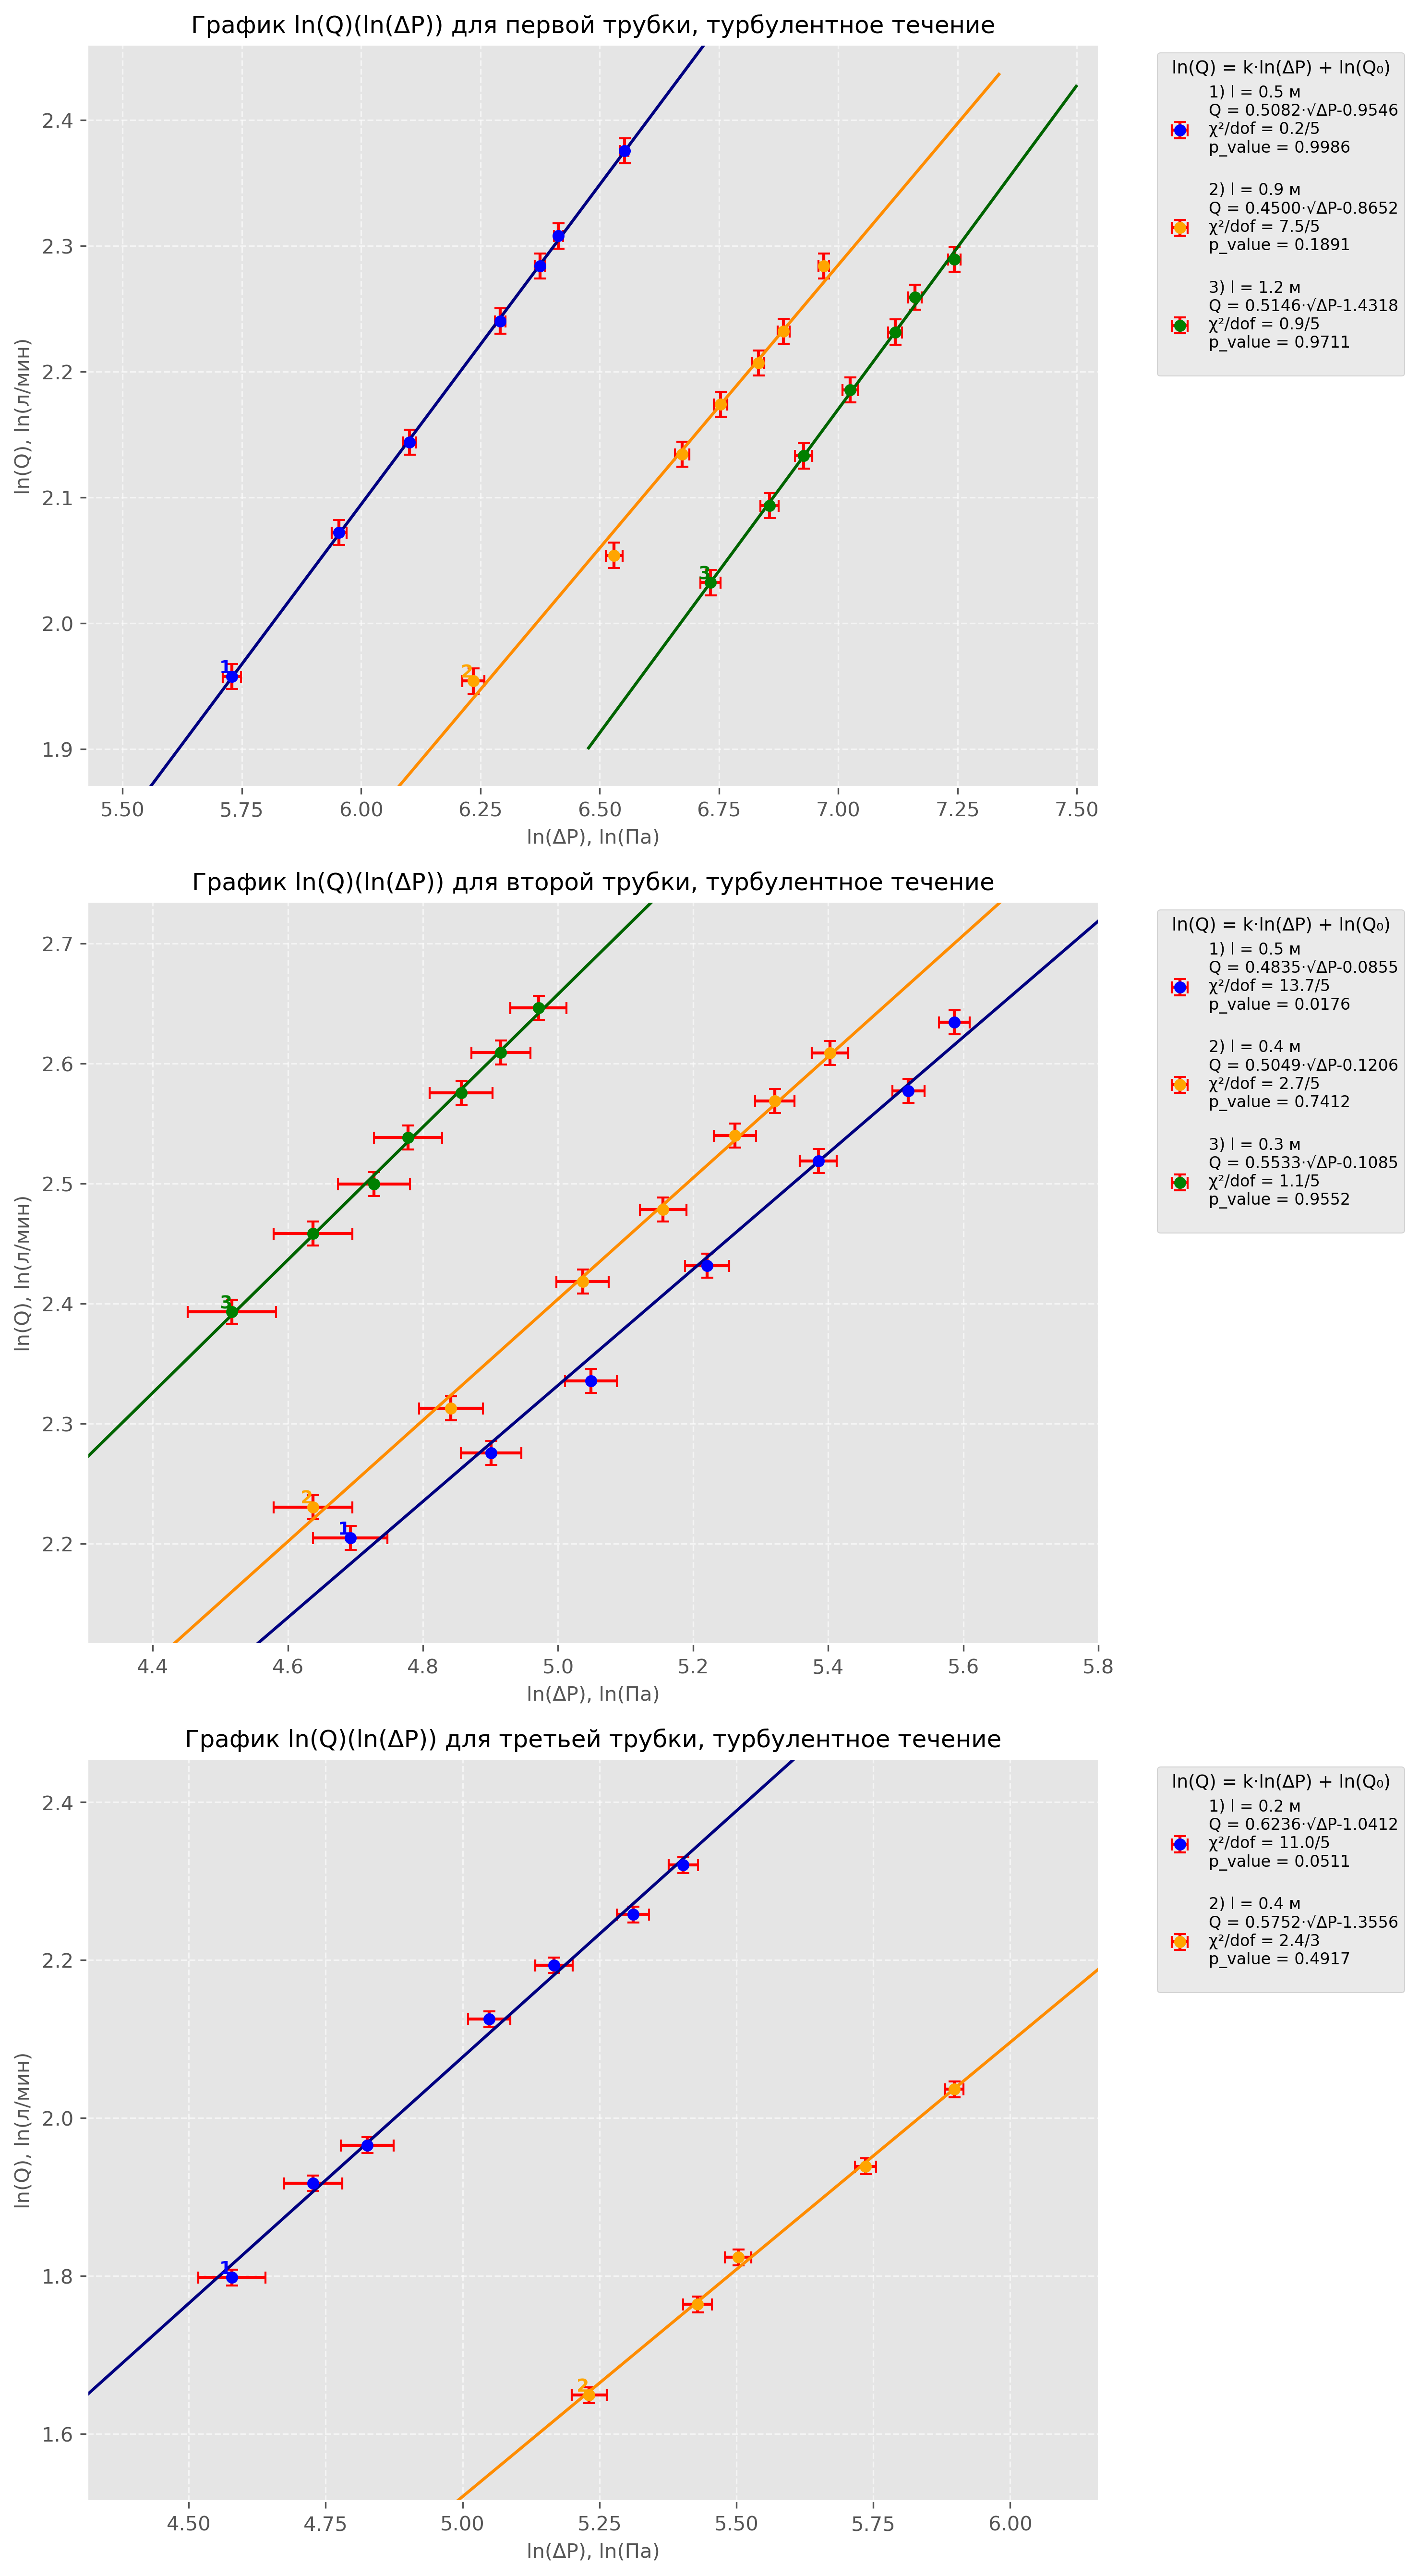
\includegraphics[width=0.75\textwidth]{Graph_loglog_4-6_tur.png}}
\caption[]{\label{} Графики №7-9 $Q(\Delta P)$ в двойном логарифмическом масштабе при турбулентном течении}
\end{figure}
По ламинарным участкам с помощью угловых коэффициентов найдем вязкость воздуха $\eta$

\begin{equation*}
	\eta = \frac{\pi R^4}{8kl} = \frac{3,1415 \cdot (\frac{3,9}{2} \cdot 10^{-3})^4 \cdot 60 \cdot 10^3}{8\cdot 0,034 \cdot 0,5} \approx 2.007 \cdot 10^{-5} \, \text{Па} \cdot \text{с}
\end{equation*}
\begin{equation*}
	\sigma_\eta = \eta \sqrt{\left(\frac{4\sigma_R}{R}\right)^2 + \left(\frac{\sigma_k}{k}\right)^2} = 2.007 \cdot 10^{-5} \sqrt{(0,05)^2 + (0,008)^2} \approx 0,206 \cdot 10^{-5} \, \text{Па} \cdot \text{с}
\end{equation*}

\begin{table}[h!]
    \centering
    \begin{tabular}{|c|c|c|}
        \hline
        $\eta, \cdot 10^{-5} \text{Па} \cdot \text{с}$ & $\sigma_\eta, \cdot 10^{-5} \text{Па} \cdot \text{с}$ & $\varepsilon_\eta, \%$ \\
        \hline
        2.007 & 0.206 & 10.29 \\ \hline
        1.951 & 0.201 & 10.28 \\ \hline
        1.926 & 0.198 & 10.28 \\ \hline
        1.984 & 0.205 & 10.32 \\ \hline
        2.213 & 0.228 & 10.30 \\ \hline
        2.140 & 0.220 & 10.29 \\ \hline
        0.807 & 0.084 & 10.41 \\ \hline
        0.777 & 0.080 & 10.30 \\ \hline
    \end{tabular}
    \captionof{table}{Таблица 17. Экспериментальные значения коэффициентов воздуха для серий 1-8.}
\end{table}

\item Для определения границы перехода от ламинарного участка к турбулентному найдем точки пересечения графика зависимости для ламинарного и турбулентного течения. Однако, как показали результаты, эти точки в некоторых сериях значительно меньше рассчитанных предварительно, поэтому лучше построить линейную зависимость для точек турбулентного течения (эта прямая будет секущей для графика и линейным приближением) и уже с помощью нее найдем точки пересечения.
\begin{figure}[h!]
\centering{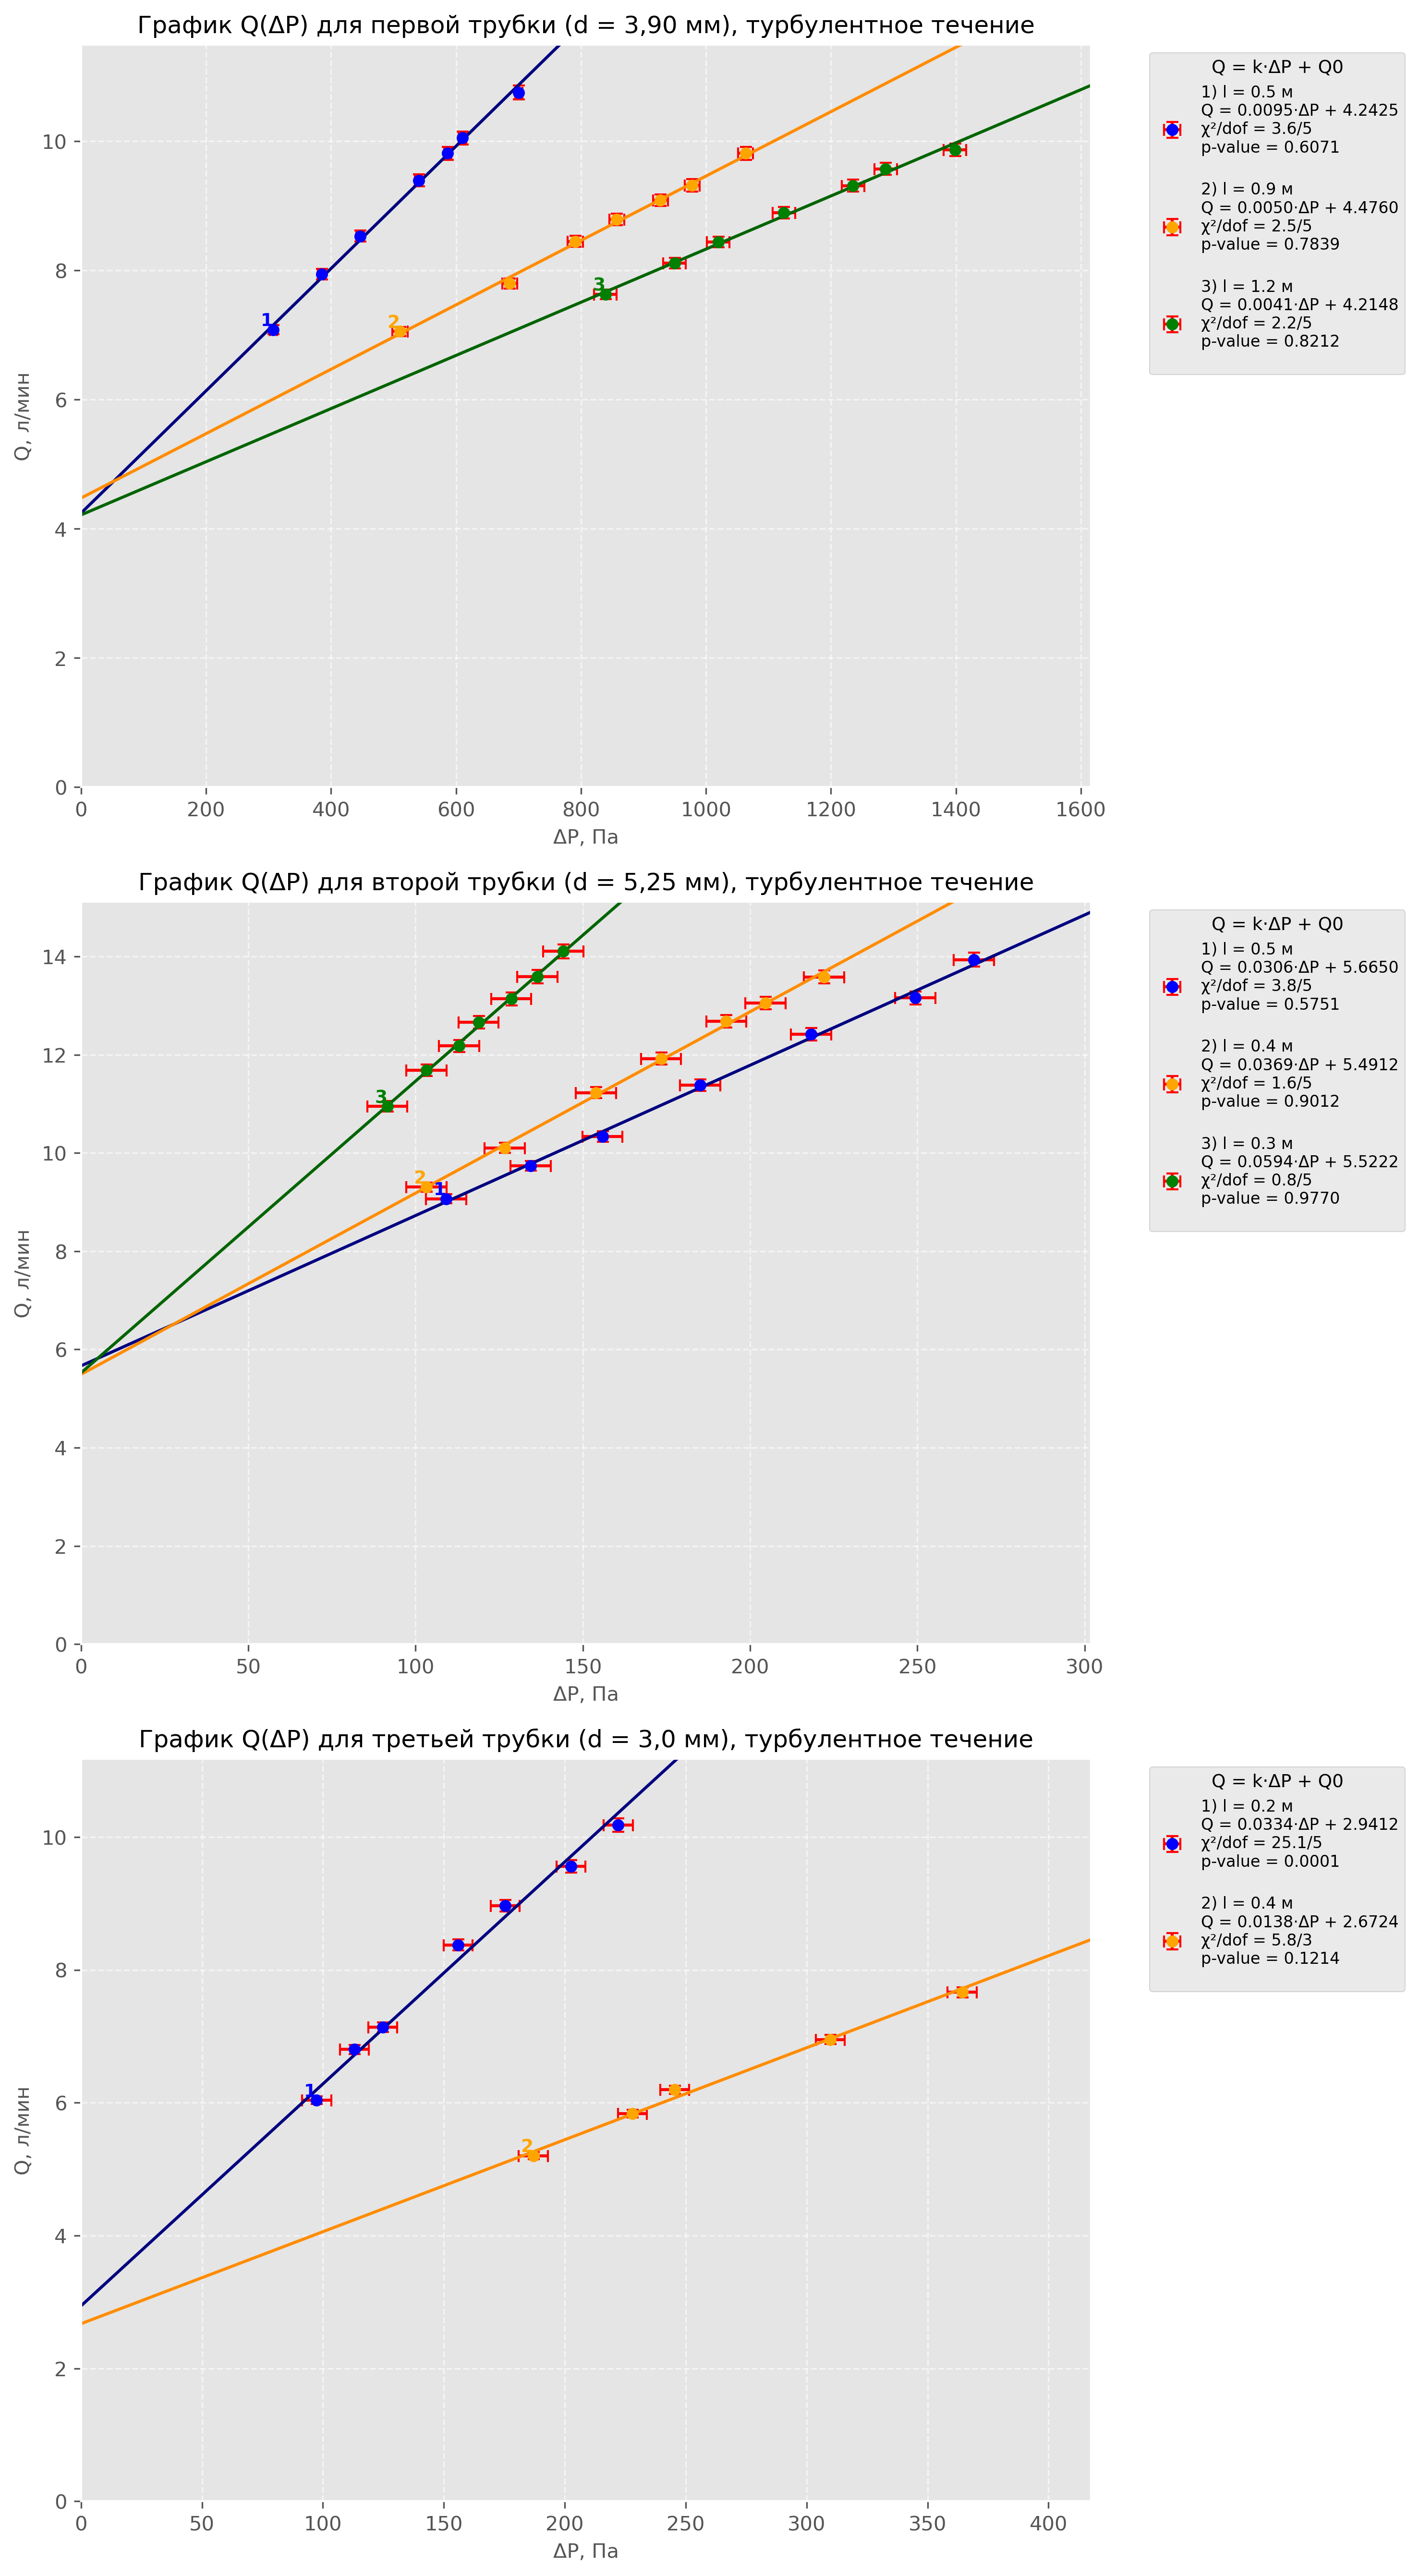
\includegraphics[width=0.75\textwidth]{Graph_4-6_lin.png}}
\caption[]{\label{} Графики №10-12 Линейная зависимость $Q(\Delta P)$ при турбулентном течении}
\end{figure}
\clearpage
\begin{figure}[h!]
\centering{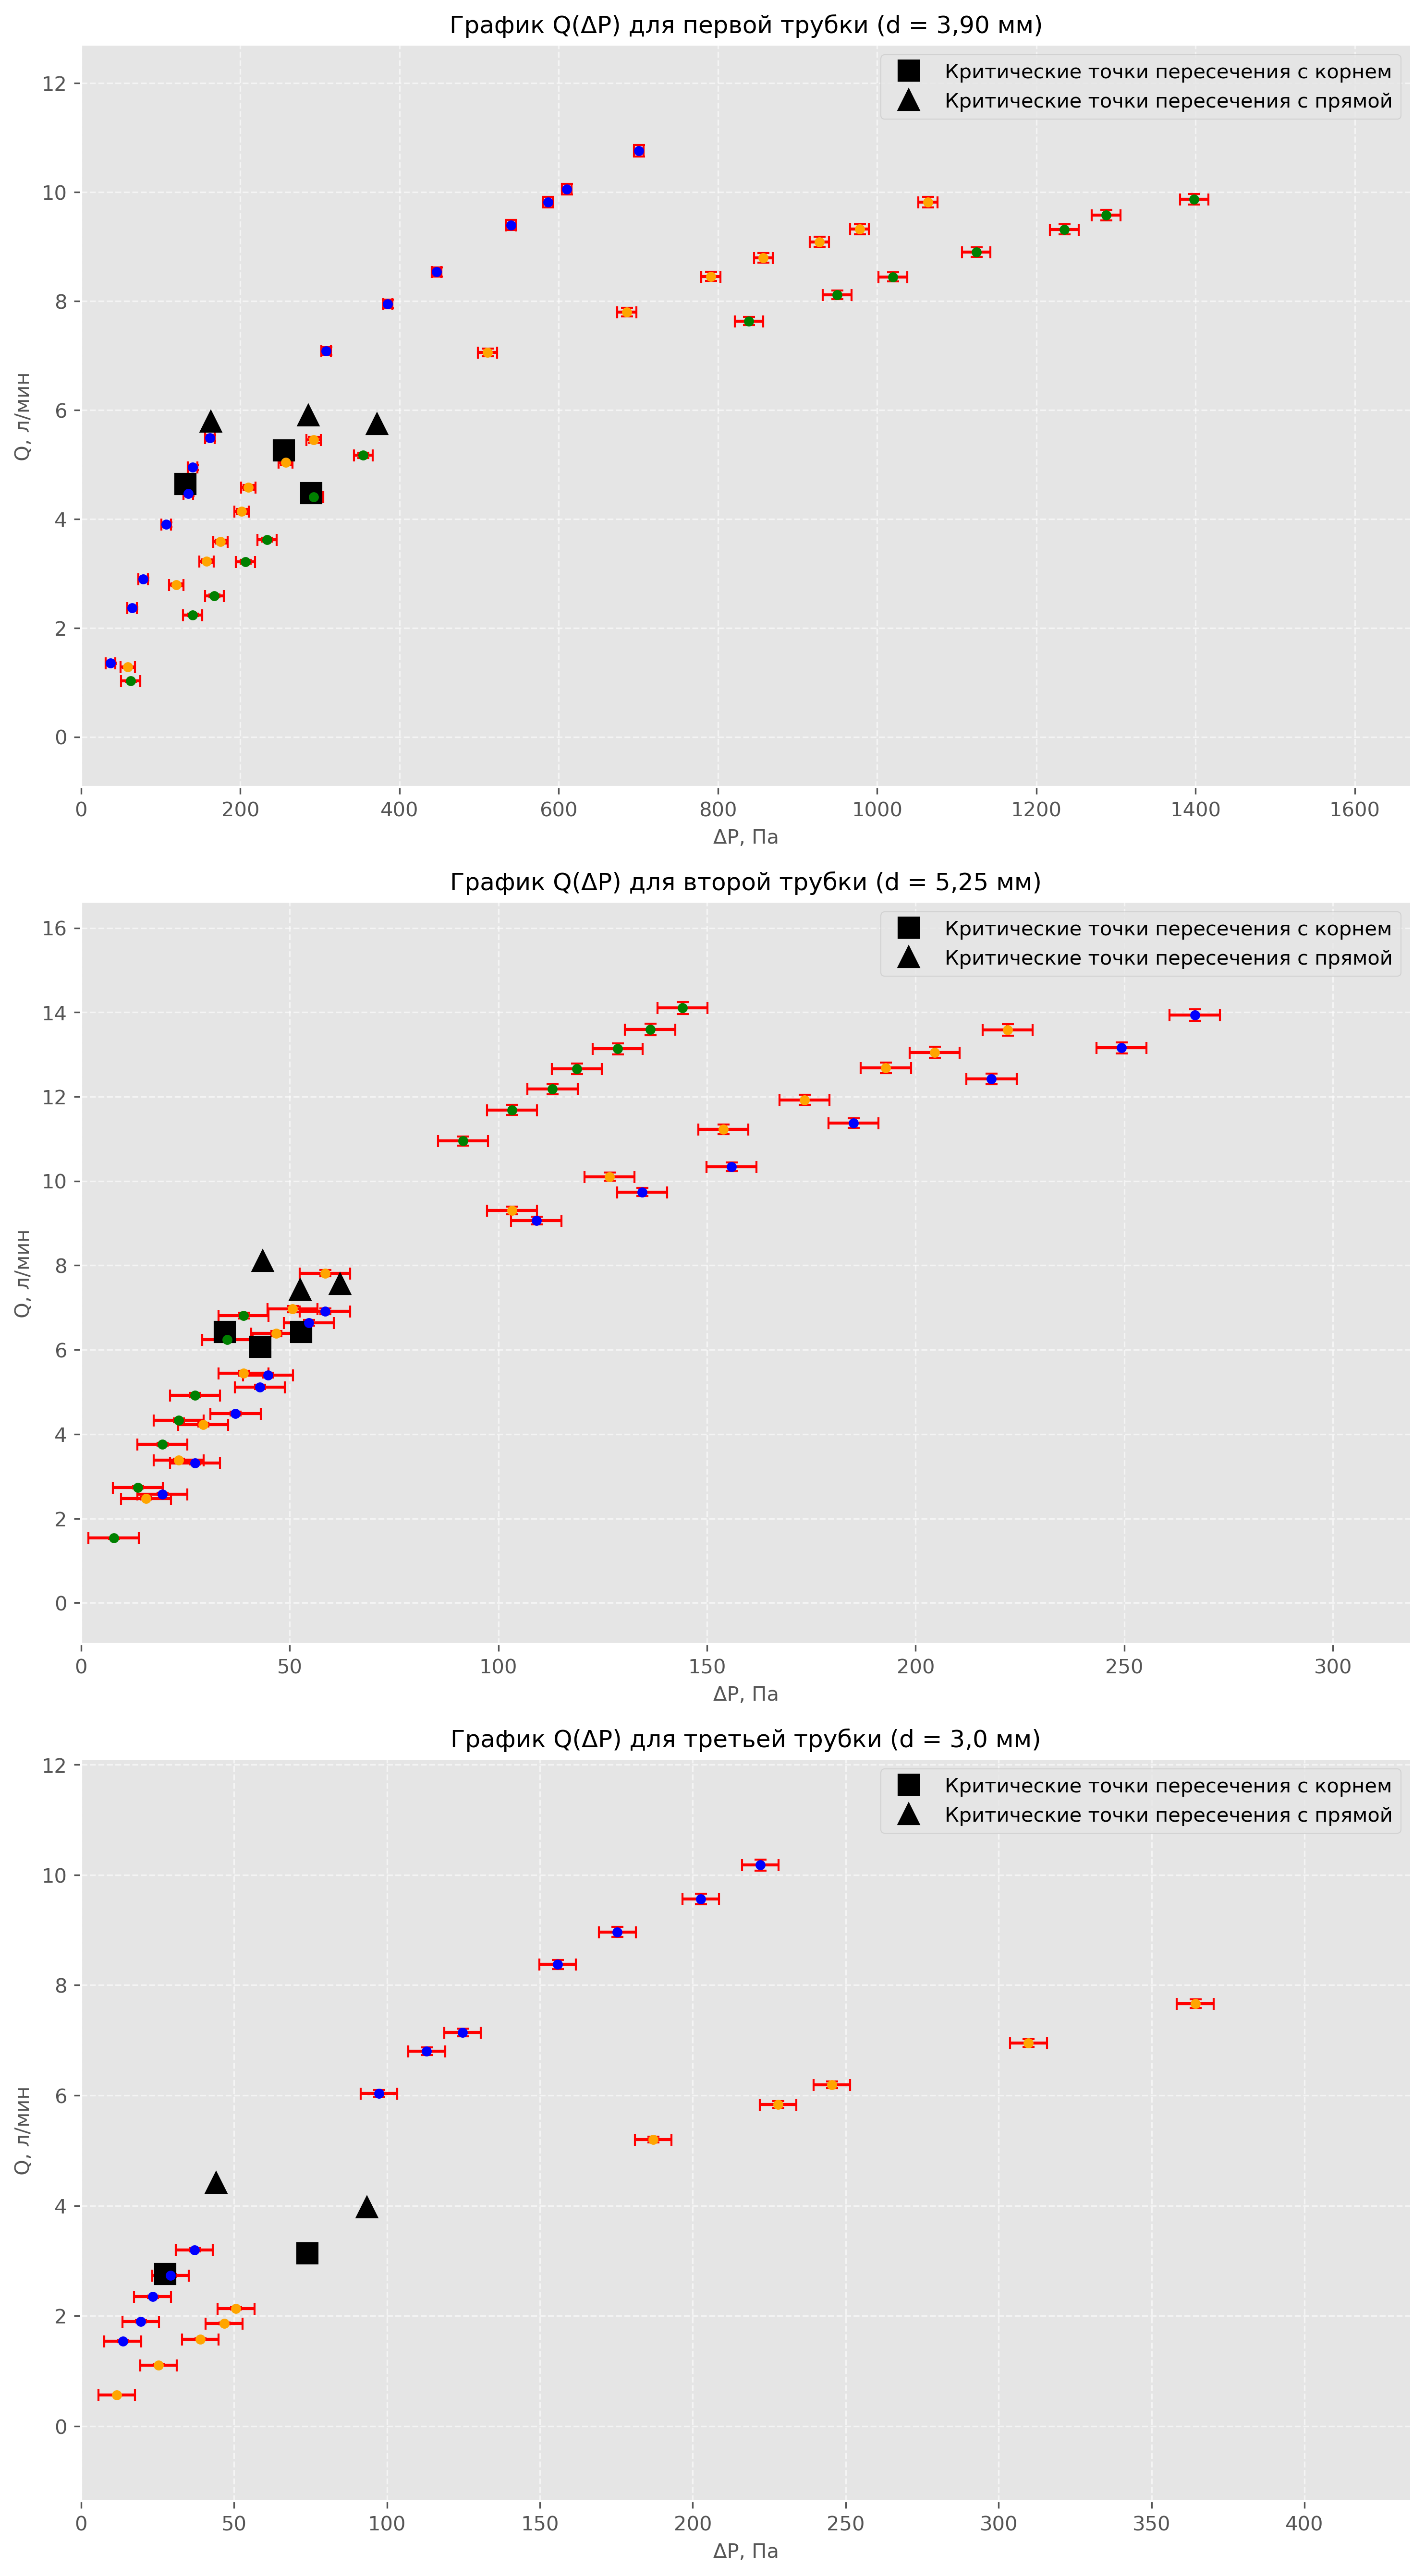
\includegraphics[width=0.75\textwidth]{All_points.png}}
\caption[]{\label{} График №13-15 $Q(\Delta P)$ с границами перехода от ламинарного участка к турбулентному}
\end{figure}

По границами перехода от ламинарного участка к турбулентному рассчитаем число Рейнольдса $Re_\text{кр}$
\begin{equation*}
	Re_\text{кр} = \frac{P \mu_{\text{воз}} Q_\text{кр}}{R_\text{газ}T \eta \pi R}
\end{equation*}

\begin{table}[h!]
    \centering
    \begin{tabular}{|c|c|}
        \hline
        \textnumero & $Re_\text{кр}$ \\
        \hline
        1 &908 \\ \hline
        2 &952 \\ \hline
        3 &939 \\ \hline
        4 & 892 \\ \hline
        5 & 785 \\ \hline
        6 &886 \\ \hline
        7 &2239 \\ \hline
        8 &2089 \\
        \hline
    \end{tabular}
    \captionof{table}{Таблица 18. Критические значений числа Рейнольдса для серий 1-8.}
\end{table}

Рассчитаем вязкость воздуха в комнтае с учетом параметров окружающей среды. Вязксоть смеси находится по приближенной формуле как
\begin{equation*}
	\eta = \omega_{\text{с.в.}}\eta_{\text{с.в.}} + \omega_{\text{пар}}\eta_{\text{пар}},
\end{equation*}
где - $\omega_{\text{с.в.}}$ и $\omega_{\text{пар}}$ - молярные доли газов. Давление насыщеного водяного пара при нашей температуре $P_{\text{нас}} \approx 3780$ Па. Тогда
\begin{equation*}
	\omega_{\text{пар}} = \frac{\varphi P_{\text{нас}}}{P_{\text{комн}}} \approx 0,0088,
\end{equation*}
\begin{equation*}
	\omega_{\text{с.в.}} = 1 - \omega_{\text{пар}} \approx 0,9912.
\end{equation*}
По табличным значениям коэффициентов вязкости для сухого воздуха и водяного пара, взятым из книги Лабораторный практикум по общей физике Том I термодинамика и молекулярная физика под редакцией Максимычева, найдем итоговое табличное значение для вязкости воздуха в комнате
\begin{equation*}
	\eta = 0,9912 \cdot 1,840 + 0,0088 \cdot 0,975 = 1,832 \cdot 10^{-5} \text{ Па} \cdot \text{с}
\end{equation*}
Табличное значение воздуха в комнате при наших условиях получилось $\eta_{\text{табл}} = 1,832 \cdot 10^{-5} \text{ Па} \cdot \text{с}$.

\item Построим график экспериментальных зависимостей, отложив по оси абсцисс Рейнольдса $Re$, а по оси ординат — обезразмеренный перепад давления $\psi = \frac{R^5\Delta P R_{\text{газ}}T\pi^2}{P\mu_{\text{воз}}lQ^2}$.
\clearpage
\begin{figure}[h!]
\centering{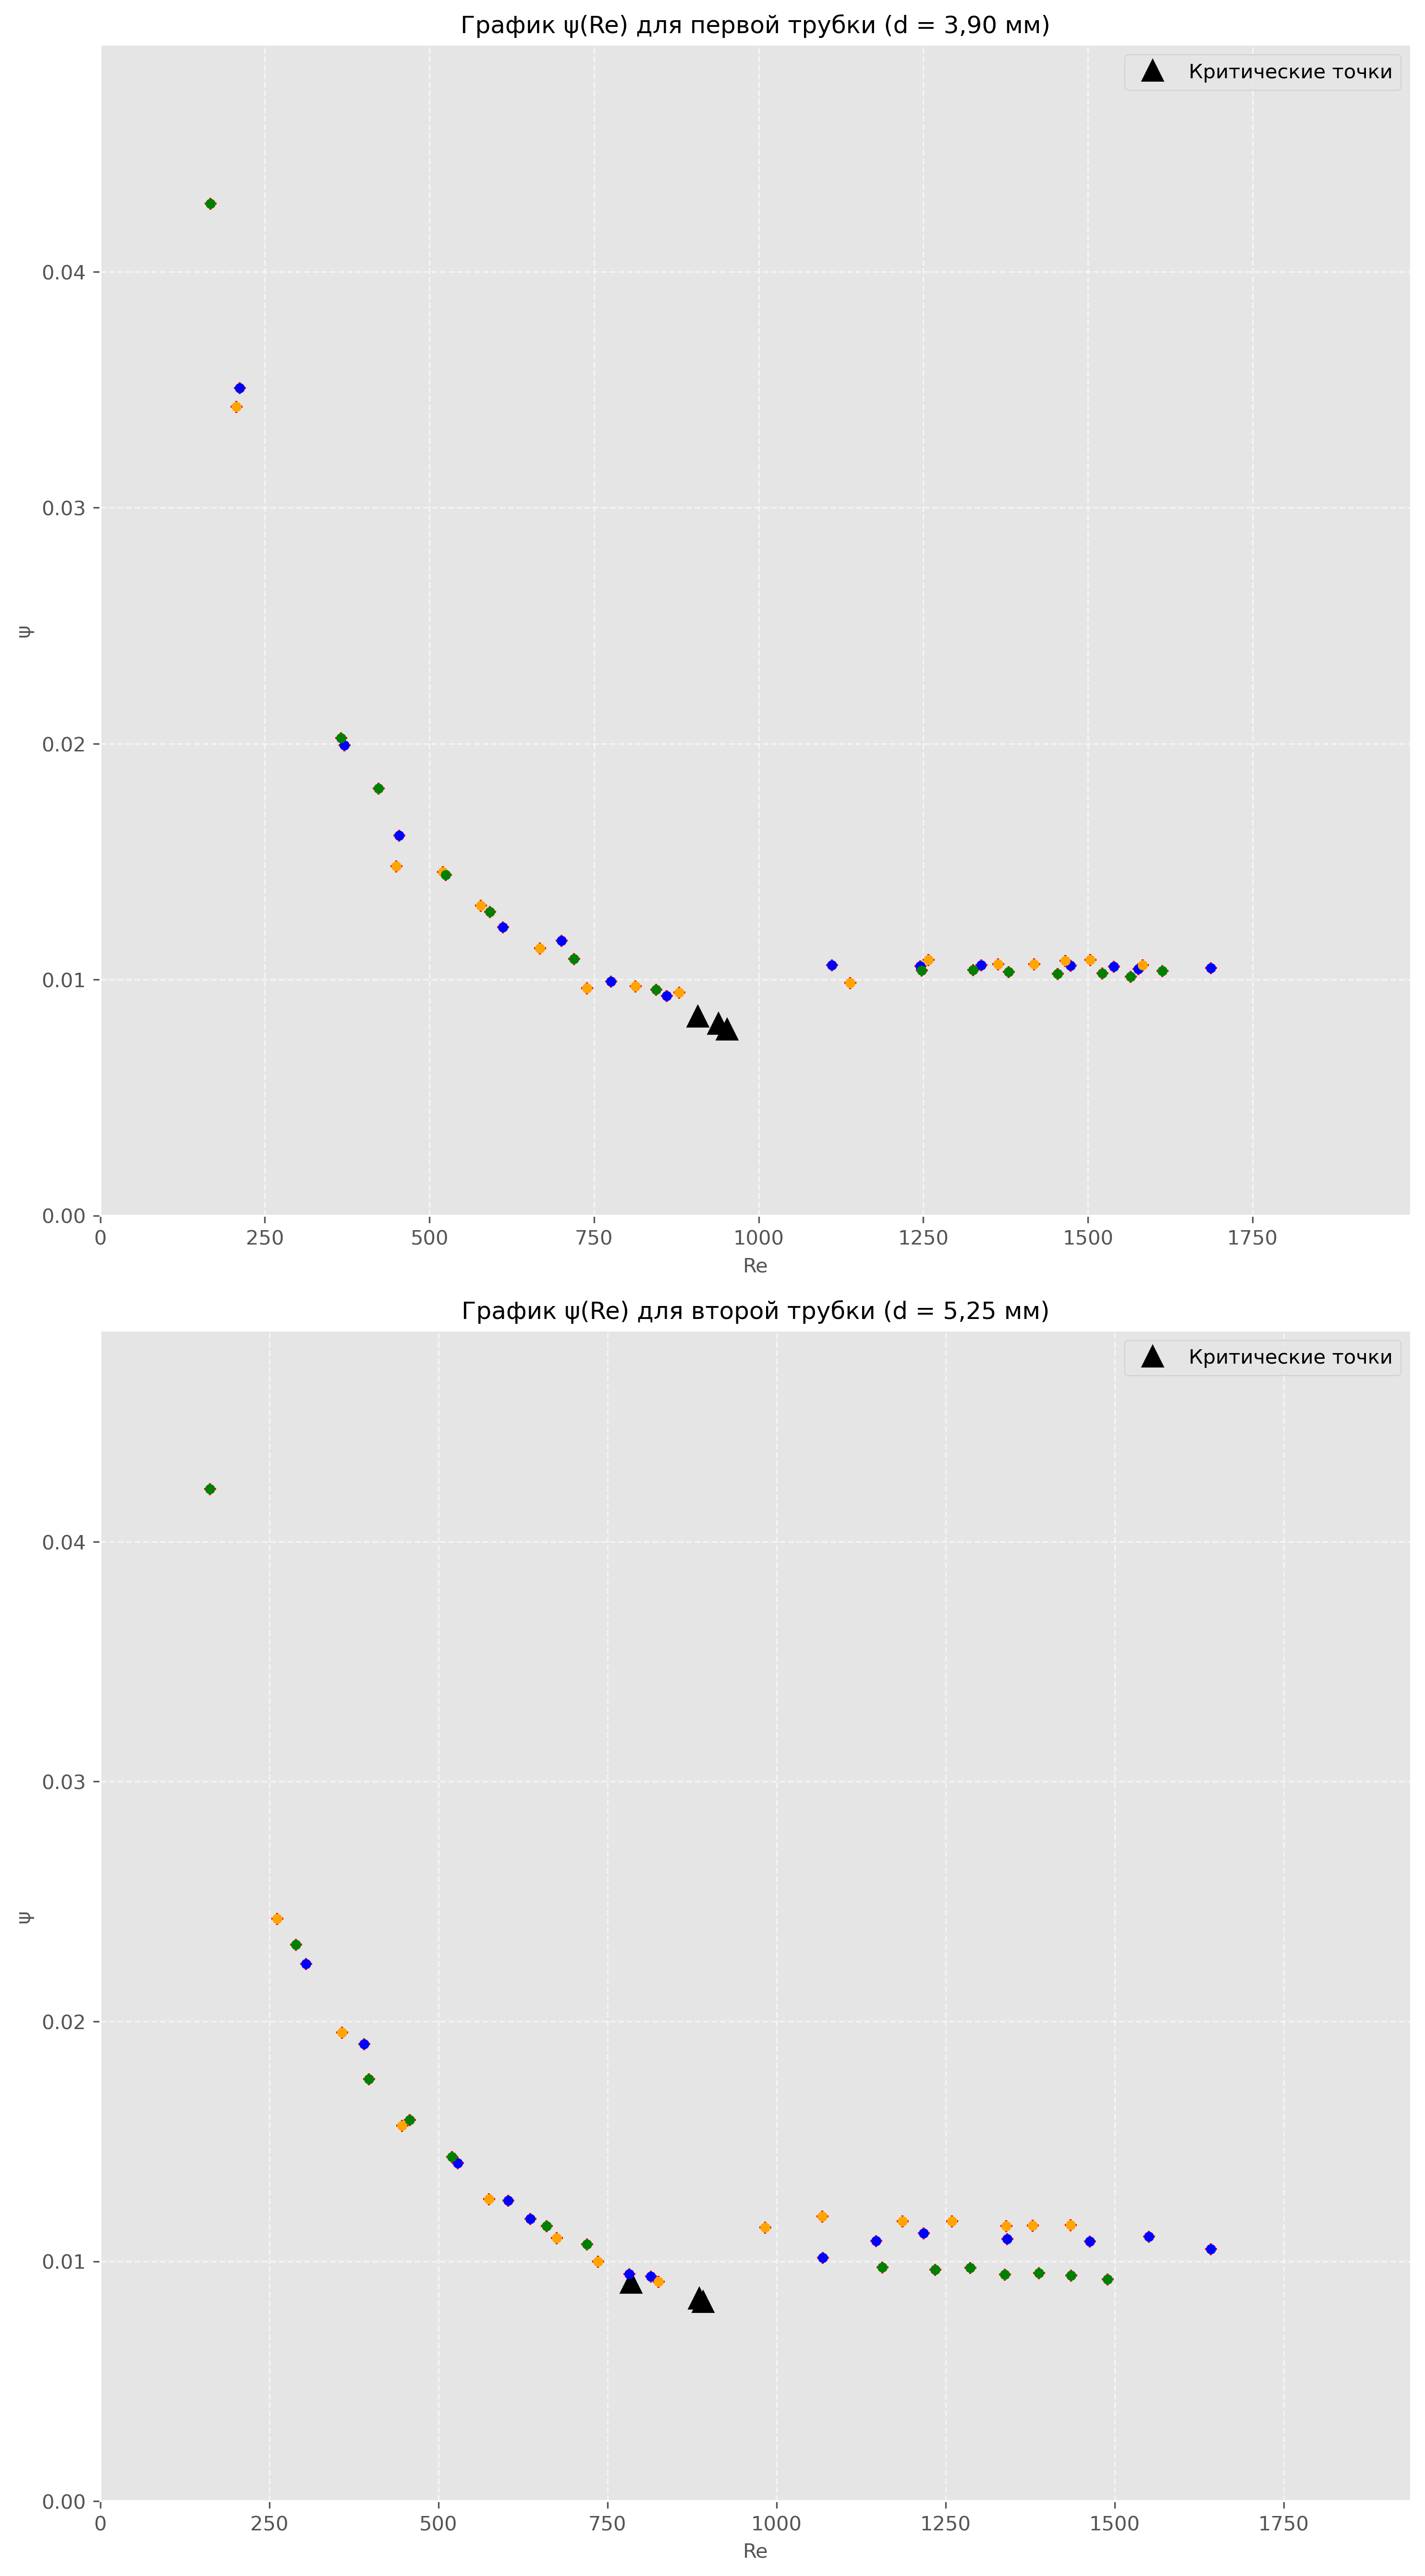
\includegraphics[width=0.75\textwidth]{All_points_psi_re.png}}
\caption[]{\label{} Графики №16-17 Зависимость $\psi(Re)$ с границами перехода от ламинарного участка к турбулентному}
\end{figure}
По графику видно, что ламинарный участок похож на график гиперболы. Убедимся в этом, построив двойной логарифмический масштаб.
\begin{figure}[h!]
\centering{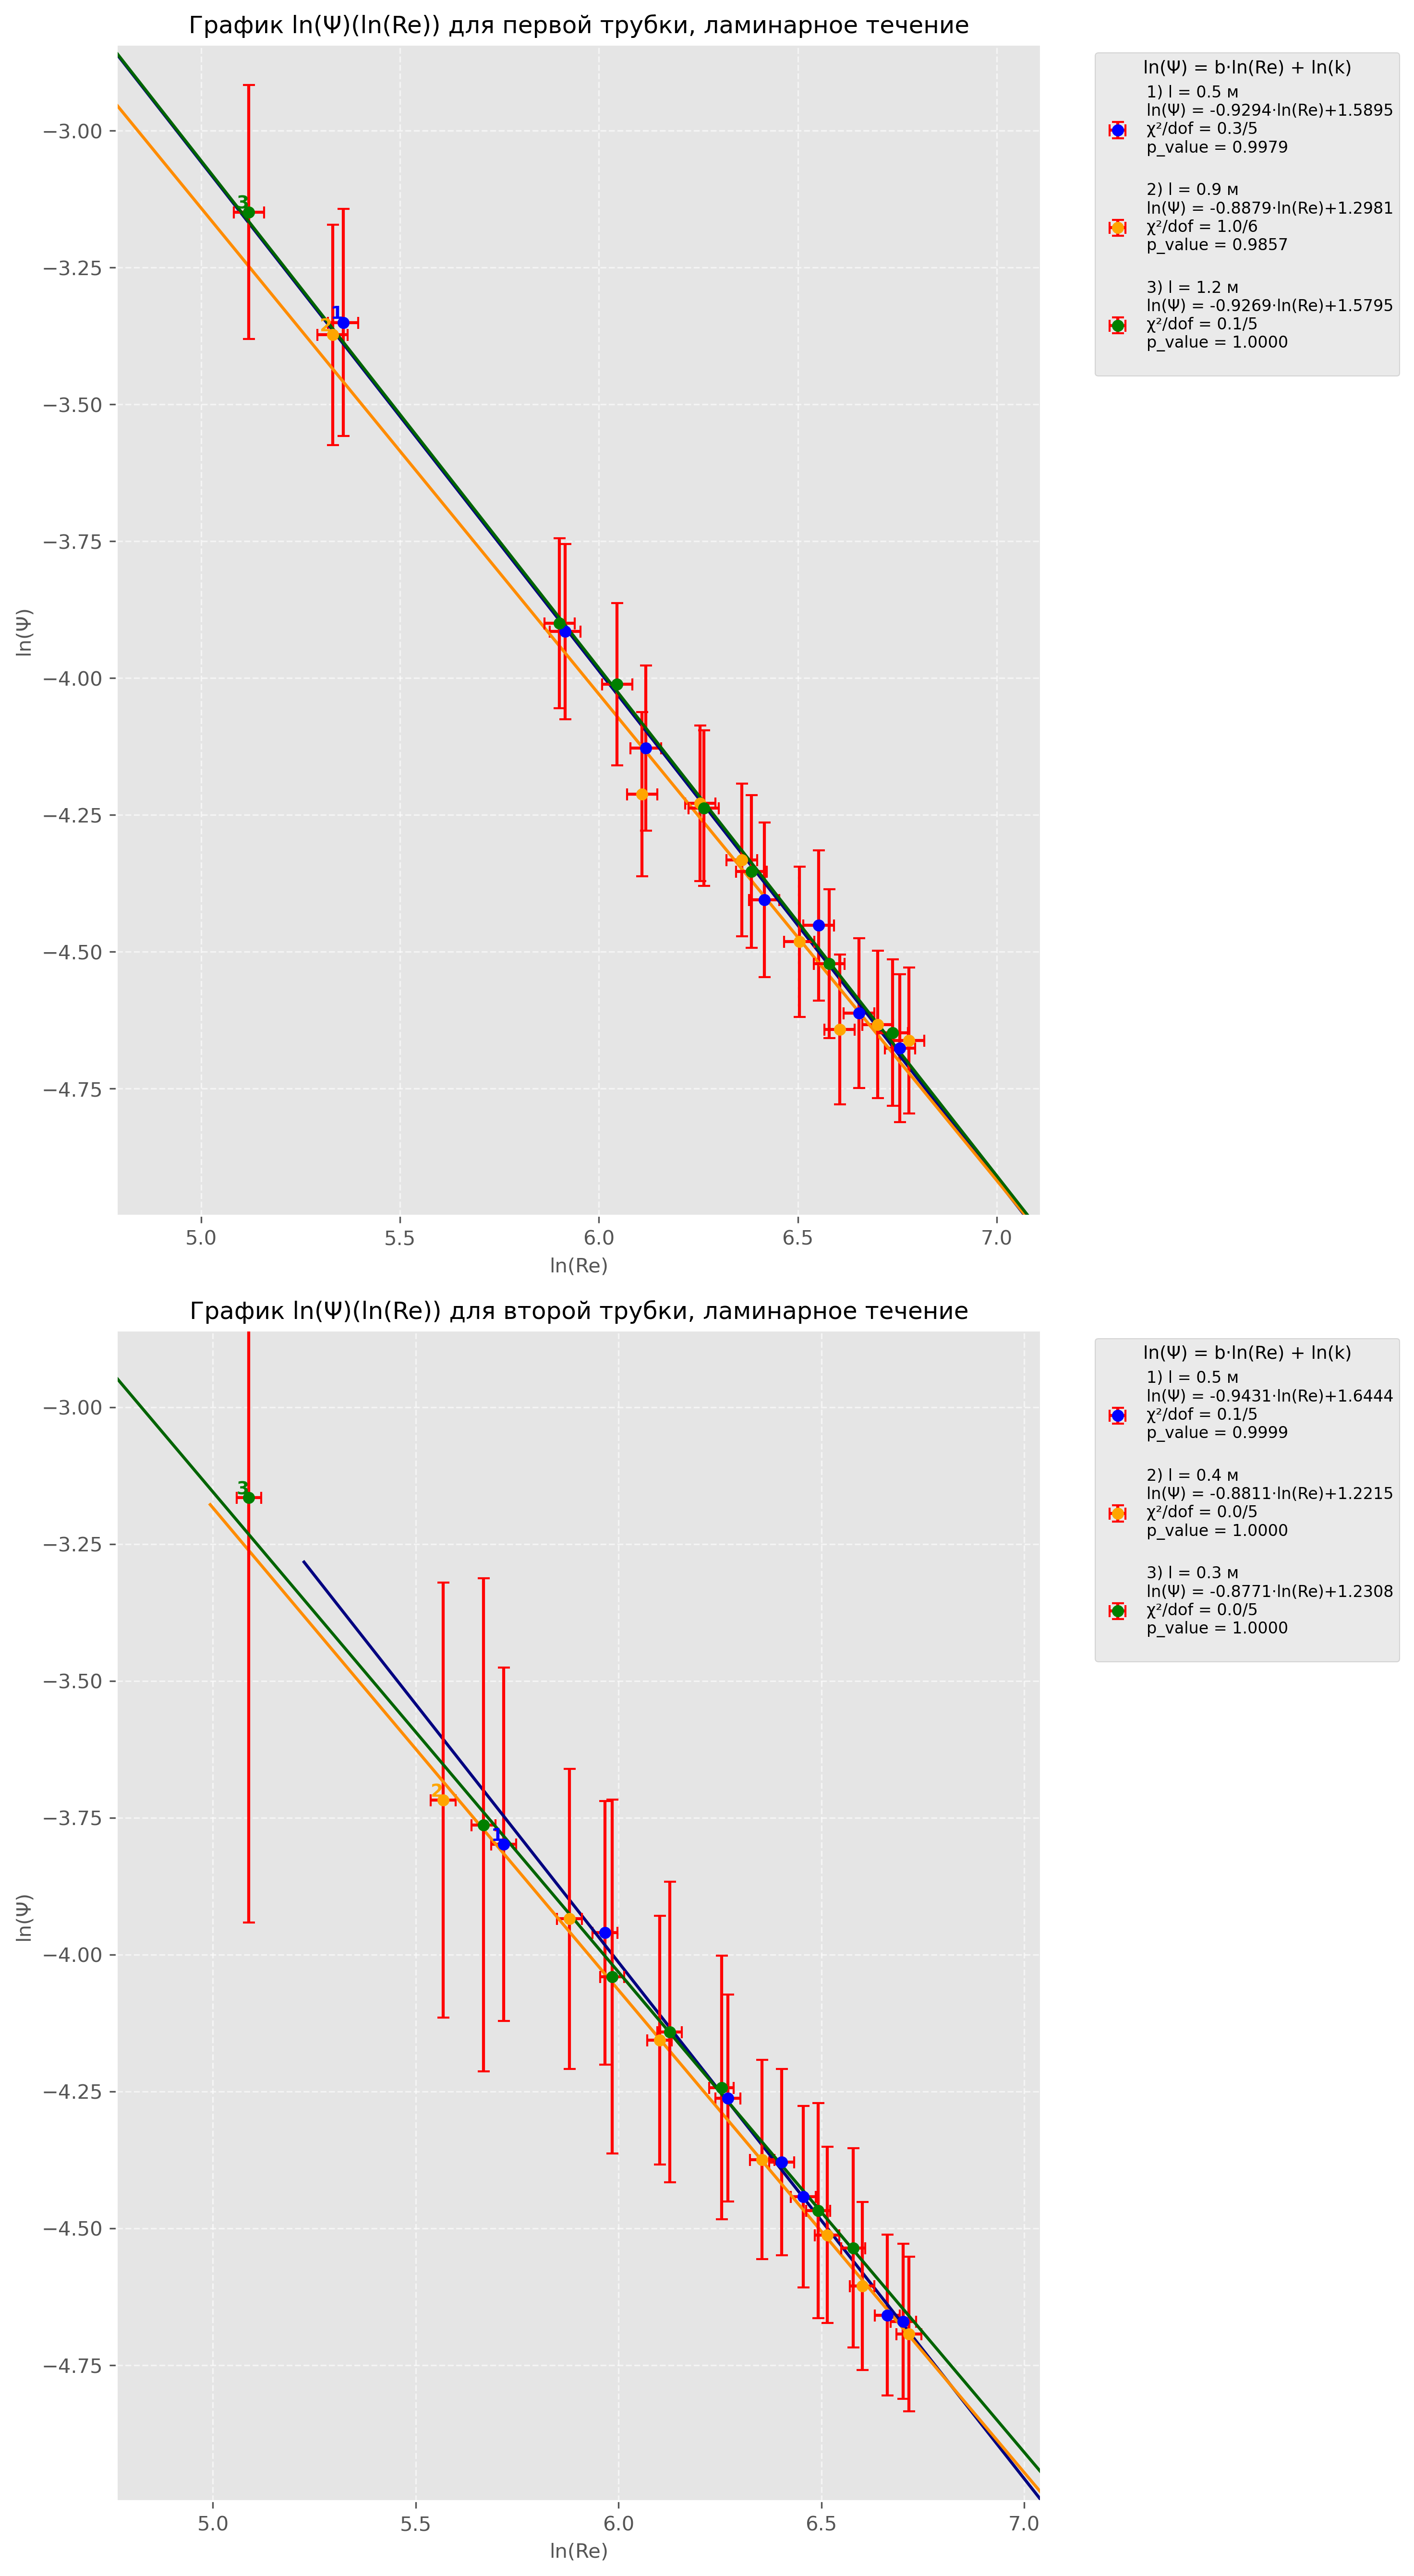
\includegraphics[width=0.7\textwidth]{Graph_loglog_psi_re_lam.png}}
\caption[]{\label{} Графики №18-19 Зависимость $\psi(Re)$ в двойном логарифмическом масштабе}
\end{figure}
\clearpage
Как видим, это действительно близкая зависимость к гиперболической с показателем $-1$. Это обосновано тем, что $\psi = \frac{8}{Re}$ для ламинарного участка, где применима формула Пуазейля. Построим эту зависимость
\begin{figure}[h!]
\centering{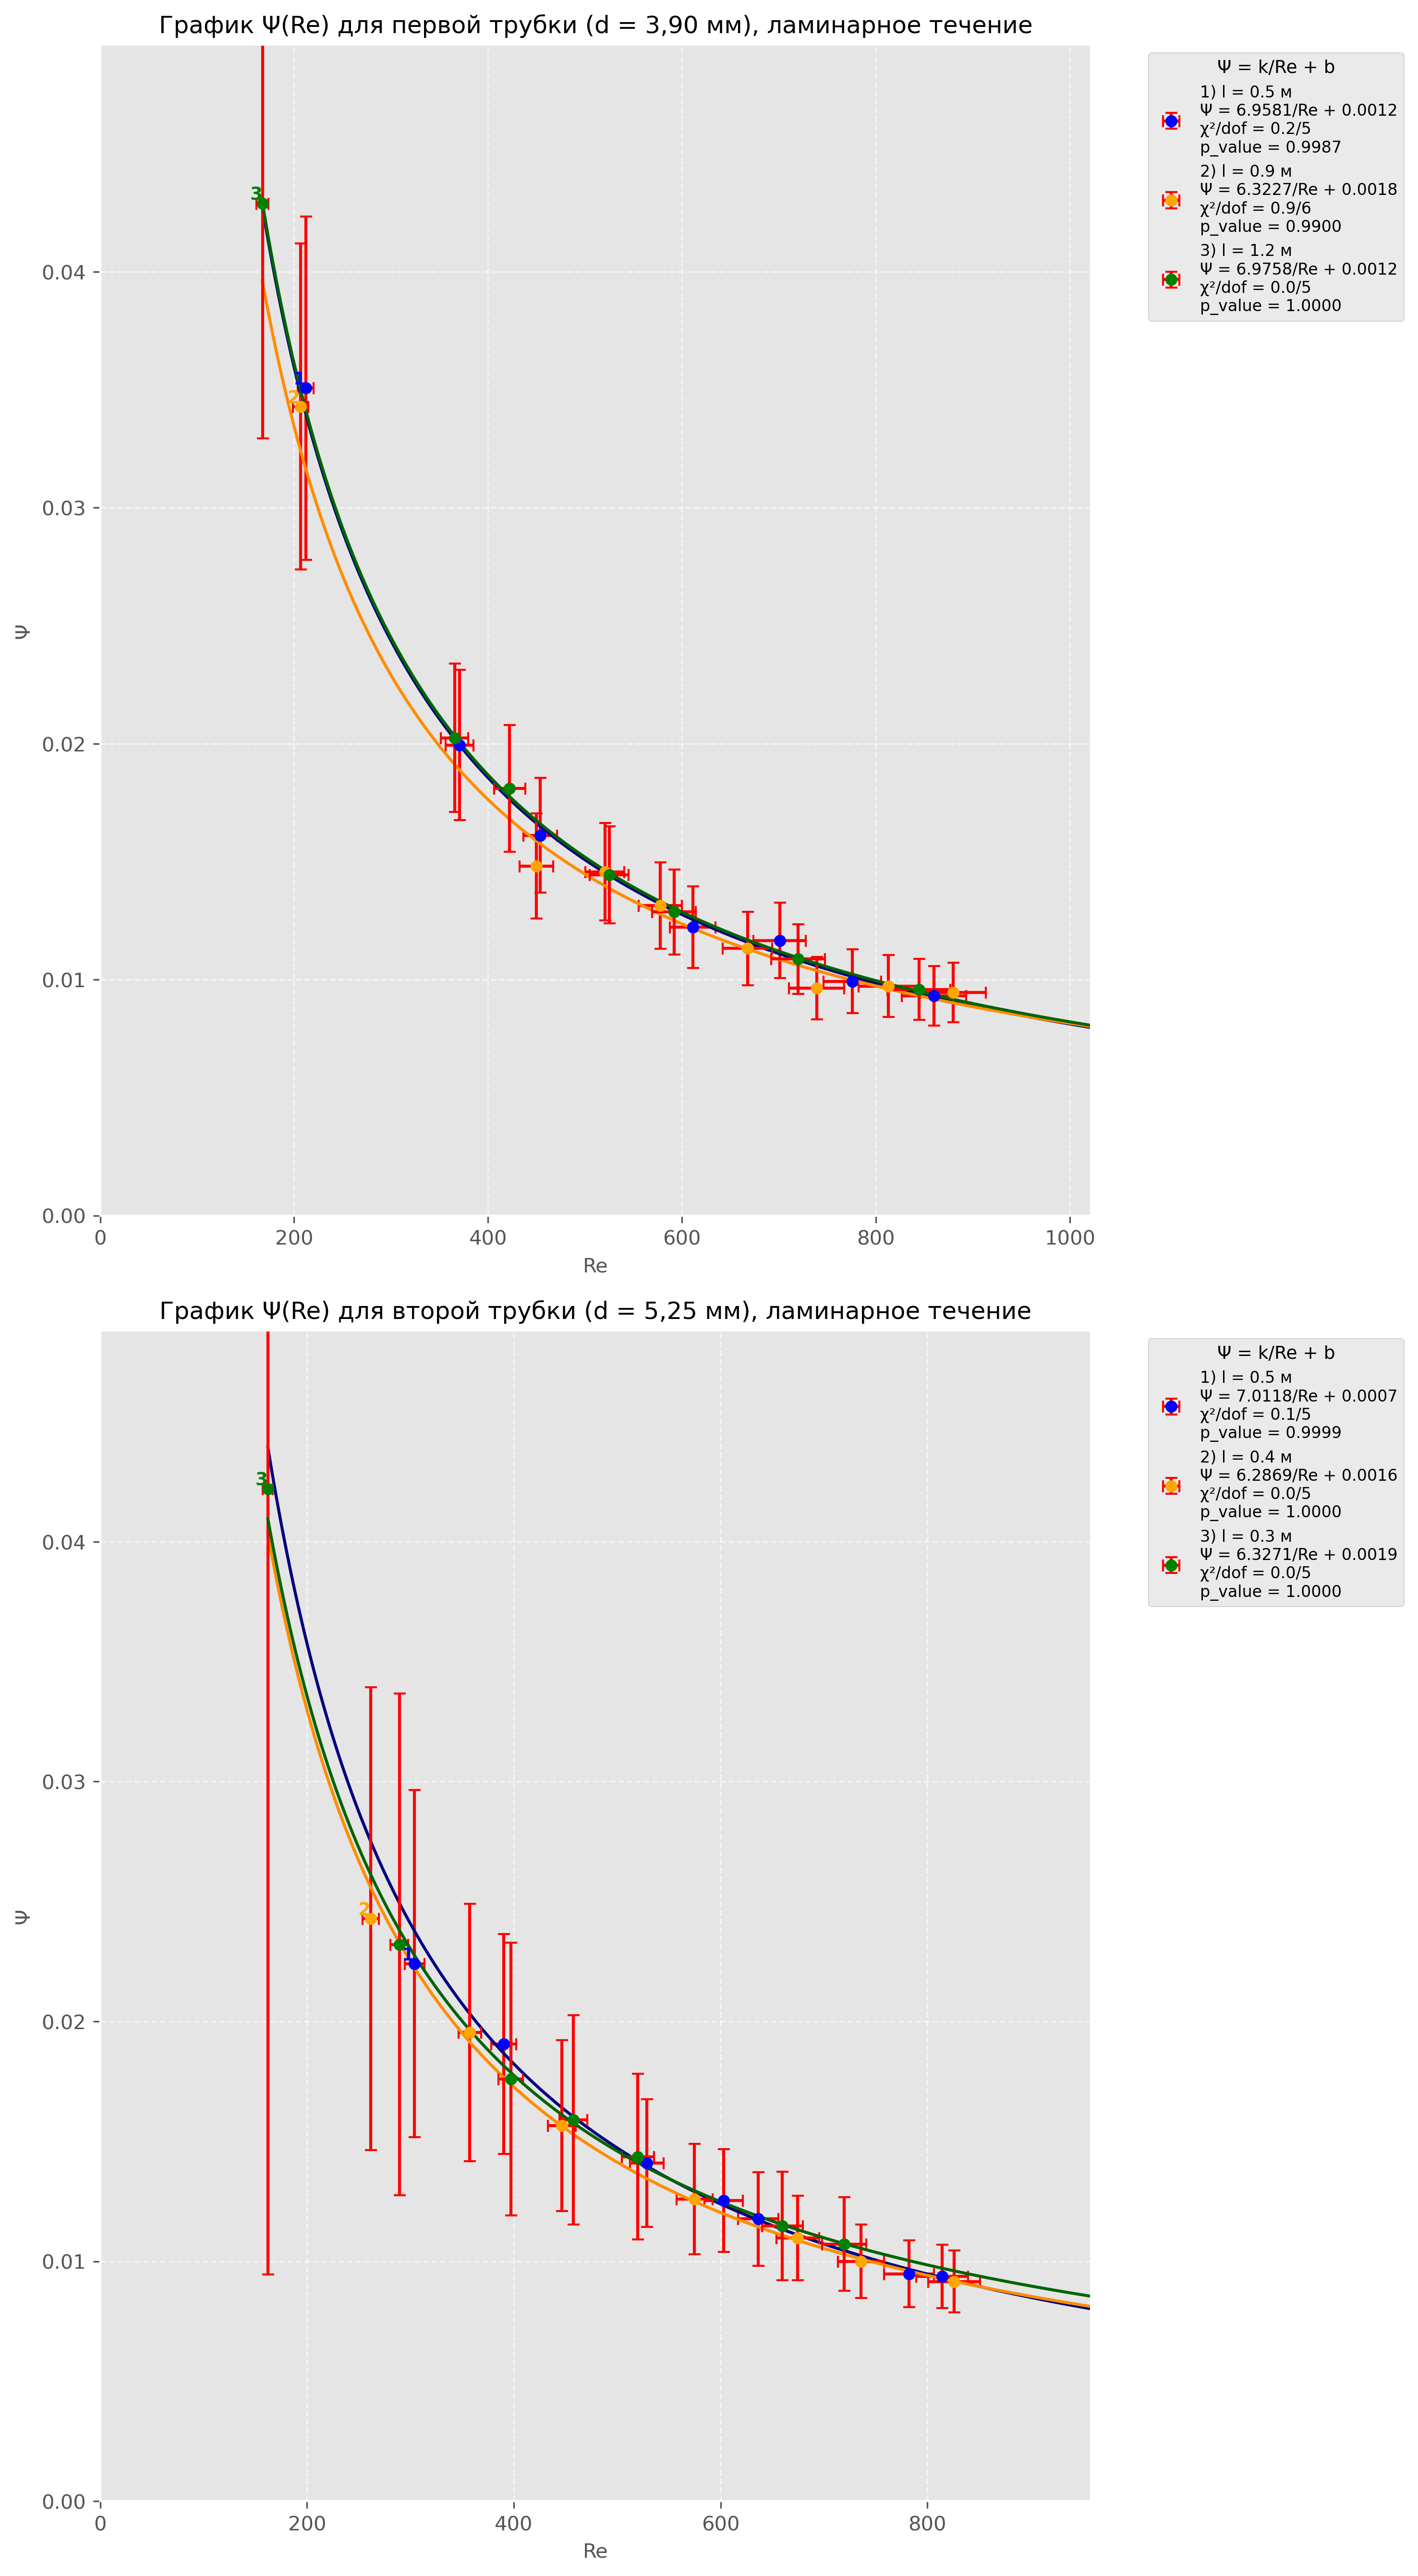
\includegraphics[width=0.70\textwidth]{Graph_psi_re_lam.png}}
\caption[]{\label{} Графики №20-21 Зависимость $\psi(Re)$ на ламинарном участке}
\end{figure}
\clearpage
\end{enumerate}
\section{Результаты и обсуждения}
\begin{enumerate}
\item По графикам 1-3 видно, что расход прямо пропорционален перепаду давления, точки хорошо ложатся на прямую при ламинарном течении. Сравним полученные экспериментально коэффициенты вязкости с табличным значением $\eta_{\text{табл}} = 1,832 \cdot 10^{-5} \, \text{Па} \cdot \text{с}$.
\begin{table}[h!]
    \centering
    \begin{tabular}{|c|c|c|c|c|}
        \hline
        $\eta, 10^{-5} \, \text{Па} \cdot \text{с}$ & $\sigma_{\eta_{\text{эксп}}}, 10^{-5} \, \text{Па} \cdot \text{с}$ & $\sigma_{\eta_{\text{табл}}}, 10^{-5} \, \text{Па} \cdot \text{с}$ & $\varepsilon_{\eta_{\text{эксп}}}, \%$ & $\varepsilon_{\eta_{\text{табл}}}, \%$ \\
        \hline
        2,007 & 0,206 & 0,175 & 10,29 & 9,53 \\ \hline
        1,951 & 0,201 & 0,119 & 10,28 & 6,48 \\ \hline
        1,926 & 0,198 & 0,094 & 10,28 & 5,11 \\ \hline
        1,984 & 0,205 & 0,152 & 10,32 & 8,28 \\ \hline
        2,213 & 0,228 & 0,381 & 10,30 & 20,78 \\ \hline
        2,140 & 0,220 & 0,307 & 10,29 & 16,76 \\ \hline
        0,807 & 0,084 & 1,025 & 10,41 & 55,95 \\ \hline
        0,777 & 0,080 & 1,055 & 10,30 & 57,60 \\ \hline
    \end{tabular}
    \captionof{table}{Таблица 19. Сравнение экспериментальных и табличных погрешностей вязкости}
\end{table}
\\
По таблице видно, что коэффициенты, полученные в сериях с трьетей трубкой отличаются более чем в 2 раза. Можем предположить, что это связано с тем, что длина трубки была меньше, чем рассчитанная длина установления давления, поэтому на этом участке течение не подчиняется закону Пуазейля. Также перепад давления на этой трубке довольно мал, что приводит к большой относительной погрешности. Именно по этим причинам в дальнейшем все рассчеты производились только для двух первых трубок. Остальные коэффициенты совпадают с табличными с хорошей точностью. Это подтверждает тот факт, что значение вязкости не зависит от диаметра трубки.
\item По графикам 4-9 можем убедиться, что при турбулентном течении расход действительно зависит от корня перепада давления. Об этом говорят значения $\frac{\chi^2}{dof}$ и $p$-value.
\item Поскольку определить точно границу перехода от ламинарного течения к турбулентному в данном опыте довольно трудно, мы воспользовались приближением и нашли эти точки как точки пересечения графиков. Однако в результате критические числа Рейнольдса для первых двух трубок действительно $\approx 10^3$.
\item Построив график $\psi(Re)$ мы убедились в том, что все точки лежат на единой кривой. С помощью графиков 16-21 видно, что на ламинарном участке $\psi$ обратно пропорционально $Re$, что говорит о применимости закона Пуазейля.
\end{enumerate}
\section{Выводы}
\begin{enumerate}
\item Провели измерения перепада давления от расхода газа для трех трубок разного диаметра и разной длины. Построили графики зависимости $Q(\Delta P)$, с помощью них нашли коэффициенты вязкости воздуха для наших параметров окружающей среды. Убедились в том, что вязкость не зависит от диаметра трубки. Оценили критические значения числа Рейнольдса. 
\item Построили зависимость безразмерного перепада давления от числа Рейнольдса. Убедились, что все точки лежат на единой кривой. Проверили применимость закона Пуазейля для ламинарного течения.
\end{enumerate}

\end{document}